\documentclass{report}

\usepackage{amsfonts}
\usepackage{amsmath}
\usepackage{amsthm}
\usepackage{hyperref}
\usepackage{tikz}
\usepackage{graphicx}
\usepackage{float}
\usepackage[utf8]{inputenc}
\usepackage{fontenc}
\usepackage[boxruled,linesnumbered]{algorithm2e}
\usepackage{booktabs}
\usepackage{multirow}

\usepackage{cleveref}

\usepackage[sorting=none, backend=bibtex]{biblatex}
\bibliography{references,rfc}

\theoremstyle{plain}
\newtheorem{theorem}{Theorem}[section]
\newtheorem{lemma}[theorem]{Lemma}
\newtheorem{proposition}[theorem]{Proposition}
\newtheorem*{corollary}{Corollary}

\theoremstyle{definition}
\newtheorem{definition}{Definition}[section]
\newtheorem{conjecture}{Conjecture}[section]
\newtheorem{example}{Example}[section]

\theoremstyle{remark}
\newtheorem*{remark}{Remark}
\newtheorem*{note}{Note}

\crefname{algocf}{alg.}{algs.}
\Crefname{algocf}{Algorithm}{Algorithms}

\title{PhD First Year  Report:\\ Information Leakage on Encrypted Sensor Network Traffic}
%\title{tinyDTLS Experiment Record [Draft]}
\author{Yan Yan}
\date{\today}

\begin{document}

\maketitle

\tableofcontents

\chapter{Introduction}

\section{Cryptography and Side Channel Attacks}
Cryptography derived from solving the problem of transmitting secret information through an insecure channel. The general principle  in modern cryptography is that the encryption and decryption algorithms are assumed to be made public and the secrecy of messages is solely relied on the secrecy of the key. 

Under this assumption, cryptographic algorithms are then designed in various ways. Some of them are derived from hard mathematical problems such as Discrete Logarithm and Elliptic Curves. Provable Security provides mathematical proofs by modelling the algorithms in an abstracted mathematical world and reduces them to hard problems; the secrecy of message is then guaranteed as long as the underlying mathematical problems are not solved.

However, when implemented in real world things can get out of control. Many factors considered difficult to be modelled mathematically can sometimes be exploited to breach the security. For example, \cite{DPA} describes a method called Differential Power Analysis which recovers the secret key using power traces measured during encryption; \cite{Cache-Timing1} and \cite{Cache-Timing2} shows that the timing information can also  reveal the secret key.

\section{Network Traffic}
The conceptional structure of today’s network is described in \cite{OSI}. Generally speaking, networks are formed by protocols which are standard agreements implemented by nodes connected to the networks. Protocols are categorised as a stack of layer with the lower ones handle the fussy transportation  problems and the higher ones the more sophisticated functional problems. 

Packet (or frame) is the unit of structured data transmitted through network at each layer. A typical format of packet is a protocol header followed by its payload. The header constitutes of several fields which contain some meta data of the packet while the payload is the actual data being transmitted. 

\begin{table}[H]
\begin{center}
{\begin{tabular}{l|l|l|}
\cline{2-3}
                  & Layer             & Example Protocols        \\ \cline{2-3} 
High            & Application Layer & HTTP / SMTP / NTP        \\ \cline{2-3} 
  & Secure Layer      & TLS / SSL / DTLS         \\ \cline{2-3} 
              & Transport Layer   & TCP / UDP / SCTP         \\ \cline{2-3} 
              & Network Layer     & IPv4 / IPv6 / 6lowPAN    \\ \cline{2-3} 
               & Data Link Layer   & IEEE 802.3 / IEEE 802.11 \\ \cline{2-3} 
Low                 & Physical Layer    &  Bluetooth / DSL        \\ \cline{2-3} 
\end{tabular}
}
\end{center}
\caption{A Simplified 6 Layer Model}
\label{Tbl: OSI}
\end{table}

Packet of protocols are organised recursively, i.e. headers of upper protocols is embedded into the payload of lower protocols. When a packet (or frame) arrives a node on the network, the headers are decapsulated sequentially from the lowest layer to the highest. Conceptional speaking, the content of a payload should be transparent to the protocols beneath. For instance, a router may only decapsulate a packet no higher than IP layer and has no concern about everything above.

\begin{figure}[H]
\centering
\resizebox{12cm}{!}
{% Graphic for TeX using PGF
% Title: /home/yy12135/Writings/First-year-review_20150422/Pics/HeaderPayload.dia
% Creator: Dia v0.97.2
% CreationDate: Wed Apr  1 16:51:21 2015
% For: yy12135
% \usepackage{tikz}
% The following commands are not supported in PSTricks at present
% We define them conditionally, so when they are implemented,
% this pgf file will use them.
\ifx\du\undefined
  \newlength{\du}
\fi
\setlength{\du}{15\unitlength}
\begin{tikzpicture}
\pgftransformxscale{1.000000}
\pgftransformyscale{-1.000000}
\definecolor{dialinecolor}{rgb}{0.000000, 0.000000, 0.000000}
\pgfsetstrokecolor{dialinecolor}
\definecolor{dialinecolor}{rgb}{1.000000, 1.000000, 1.000000}
\pgfsetfillcolor{dialinecolor}
\definecolor{dialinecolor}{rgb}{1.000000, 1.000000, 1.000000}
\pgfsetfillcolor{dialinecolor}
\fill (15.787500\du,22.000000\du)--(15.787500\du,23.900000\du)--(20.000000\du,23.900000\du)--(20.000000\du,22.000000\du)--cycle;
\pgfsetlinewidth{0.100000\du}
\pgfsetdash{}{0pt}
\pgfsetdash{}{0pt}
\pgfsetmiterjoin
\definecolor{dialinecolor}{rgb}{0.000000, 0.000000, 0.000000}
\pgfsetstrokecolor{dialinecolor}
\draw (15.787500\du,22.000000\du)--(15.787500\du,23.900000\du)--(20.000000\du,23.900000\du)--(20.000000\du,22.000000\du)--cycle;
% setfont left to latex
\definecolor{dialinecolor}{rgb}{0.000000, 0.000000, 0.000000}
\pgfsetstrokecolor{dialinecolor}
\node at (17.893750\du,23.145000\du){IP Header};
\definecolor{dialinecolor}{rgb}{1.000000, 1.000000, 1.000000}
\pgfsetfillcolor{dialinecolor}
\fill (20.000000\du,22.000000\du)--(20.000000\du,23.900000\du)--(25.000000\du,23.900000\du)--(25.000000\du,22.000000\du)--cycle;
\pgfsetlinewidth{0.100000\du}
\pgfsetdash{}{0pt}
\pgfsetdash{}{0pt}
\pgfsetmiterjoin
\definecolor{dialinecolor}{rgb}{0.000000, 0.000000, 0.000000}
\pgfsetstrokecolor{dialinecolor}
\draw (20.000000\du,22.000000\du)--(20.000000\du,23.900000\du)--(25.000000\du,23.900000\du)--(25.000000\du,22.000000\du)--cycle;
% setfont left to latex
\definecolor{dialinecolor}{rgb}{0.000000, 0.000000, 0.000000}
\pgfsetstrokecolor{dialinecolor}
\node at (22.500000\du,23.145000\du){TCP Header};
\definecolor{dialinecolor}{rgb}{1.000000, 1.000000, 1.000000}
\pgfsetfillcolor{dialinecolor}
\fill (25.000000\du,22.000000\du)--(25.000000\du,23.900000\du)--(31.000000\du,23.900000\du)--(31.000000\du,22.000000\du)--cycle;
\pgfsetlinewidth{0.100000\du}
\pgfsetdash{}{0pt}
\pgfsetdash{}{0pt}
\pgfsetmiterjoin
\definecolor{dialinecolor}{rgb}{0.000000, 0.000000, 0.000000}
\pgfsetstrokecolor{dialinecolor}
\draw (25.000000\du,22.000000\du)--(25.000000\du,23.900000\du)--(31.000000\du,23.900000\du)--(31.000000\du,22.000000\du)--cycle;
% setfont left to latex
\definecolor{dialinecolor}{rgb}{0.000000, 0.000000, 0.000000}
\pgfsetstrokecolor{dialinecolor}
\node at (28.000000\du,23.145000\du){TLS Header};
\definecolor{dialinecolor}{rgb}{1.000000, 1.000000, 1.000000}
\pgfsetfillcolor{dialinecolor}
\fill (31.000000\du,22.000000\du)--(31.000000\du,23.900000\du)--(40.000000\du,23.900000\du)--(40.000000\du,22.000000\du)--cycle;
\pgfsetlinewidth{0.100000\du}
\pgfsetdash{}{0pt}
\pgfsetdash{}{0pt}
\pgfsetmiterjoin
\definecolor{dialinecolor}{rgb}{0.000000, 0.000000, 0.000000}
\pgfsetstrokecolor{dialinecolor}
\draw (31.000000\du,22.000000\du)--(31.000000\du,23.900000\du)--(40.000000\du,23.900000\du)--(40.000000\du,22.000000\du)--cycle;
% setfont left to latex
\definecolor{dialinecolor}{rgb}{0.000000, 0.000000, 0.000000}
\pgfsetstrokecolor{dialinecolor}
\node at (35.500000\du,23.145000\du){......};
\pgfsetlinewidth{0.100000\du}
\pgfsetdash{}{0pt}
\pgfsetdash{}{0pt}
\pgfsetbuttcap
{
\definecolor{dialinecolor}{rgb}{0.000000, 0.000000, 0.000000}
\pgfsetfillcolor{dialinecolor}
% was here!!!
\pgfsetarrowsstart{to}
\pgfsetarrowsend{to}
\definecolor{dialinecolor}{rgb}{0.000000, 0.000000, 0.000000}
\pgfsetstrokecolor{dialinecolor}
\draw (31.000000\du,21.000000\du)--(40.000000\du,21.000000\du);
}
% setfont left to latex
\definecolor{dialinecolor}{rgb}{0.000000, 0.000000, 0.000000}
\pgfsetstrokecolor{dialinecolor}
\node[anchor=west] at (34.000000\du,20.000000\du){TLS payload};
\pgfsetlinewidth{0.100000\du}
\pgfsetdash{}{0pt}
\pgfsetdash{}{0pt}
\pgfsetbuttcap
{
\definecolor{dialinecolor}{rgb}{0.000000, 0.000000, 0.000000}
\pgfsetfillcolor{dialinecolor}
% was here!!!
\pgfsetarrowsstart{to}
\pgfsetarrowsend{to}
\definecolor{dialinecolor}{rgb}{0.000000, 0.000000, 0.000000}
\pgfsetstrokecolor{dialinecolor}
\draw (25.000000\du,19.000000\du)--(40.000000\du,19.000000\du);
}
% setfont left to latex
\definecolor{dialinecolor}{rgb}{0.000000, 0.000000, 0.000000}
\pgfsetstrokecolor{dialinecolor}
\node[anchor=west] at (31.000000\du,18.000000\du){TCP payload};
\pgfsetlinewidth{0.100000\du}
\pgfsetdash{}{0pt}
\pgfsetdash{}{0pt}
\pgfsetbuttcap
{
\definecolor{dialinecolor}{rgb}{0.000000, 0.000000, 0.000000}
\pgfsetfillcolor{dialinecolor}
% was here!!!
\pgfsetarrowsstart{to}
\pgfsetarrowsend{to}
\definecolor{dialinecolor}{rgb}{0.000000, 0.000000, 0.000000}
\pgfsetstrokecolor{dialinecolor}
\draw (20.000000\du,17.000000\du)--(40.000000\du,17.000000\du);
}
% setfont left to latex
\definecolor{dialinecolor}{rgb}{0.000000, 0.000000, 0.000000}
\pgfsetstrokecolor{dialinecolor}
\node[anchor=west] at (28.000000\du,16.000000\du){IP payload};
\pgfsetlinewidth{0.100000\du}
\pgfsetdash{{\pgflinewidth}{0.200000\du}}{0cm}
\pgfsetdash{{\pgflinewidth}{0.200000\du}}{0cm}
\pgfsetbuttcap
{
\definecolor{dialinecolor}{rgb}{0.000000, 0.000000, 0.000000}
\pgfsetfillcolor{dialinecolor}
% was here!!!
\definecolor{dialinecolor}{rgb}{0.000000, 0.000000, 0.000000}
\pgfsetstrokecolor{dialinecolor}
\draw (40.000000\du,16.000000\du)--(40.000000\du,25.000000\du);
}
\pgfsetlinewidth{0.100000\du}
\pgfsetdash{{\pgflinewidth}{0.200000\du}}{0cm}
\pgfsetdash{{\pgflinewidth}{0.200000\du}}{0cm}
\pgfsetbuttcap
{
\definecolor{dialinecolor}{rgb}{0.000000, 0.000000, 0.000000}
\pgfsetfillcolor{dialinecolor}
% was here!!!
\definecolor{dialinecolor}{rgb}{0.000000, 0.000000, 0.000000}
\pgfsetstrokecolor{dialinecolor}
\draw (31.000000\du,20.000000\du)--(31.000000\du,25.000000\du);
}
\pgfsetlinewidth{0.100000\du}
\pgfsetdash{{\pgflinewidth}{0.200000\du}}{0cm}
\pgfsetdash{{\pgflinewidth}{0.200000\du}}{0cm}
\pgfsetbuttcap
{
\definecolor{dialinecolor}{rgb}{0.000000, 0.000000, 0.000000}
\pgfsetfillcolor{dialinecolor}
% was here!!!
\definecolor{dialinecolor}{rgb}{0.000000, 0.000000, 0.000000}
\pgfsetstrokecolor{dialinecolor}
\draw (25.000000\du,18.000000\du)--(25.000000\du,25.000000\du);
}
\pgfsetlinewidth{0.100000\du}
\pgfsetdash{{\pgflinewidth}{0.200000\du}}{0cm}
\pgfsetdash{{\pgflinewidth}{0.200000\du}}{0cm}
\pgfsetbuttcap
{
\definecolor{dialinecolor}{rgb}{0.000000, 0.000000, 0.000000}
\pgfsetfillcolor{dialinecolor}
% was here!!!
\definecolor{dialinecolor}{rgb}{0.000000, 0.000000, 0.000000}
\pgfsetstrokecolor{dialinecolor}
\draw (20.000000\du,16.000000\du)--(20.000000\du,25.000000\du);
}
\end{tikzpicture}
}
\caption{An example of headers and payloads}
\label{Fig: Header and payloads}
\end{figure}

It might be difficult in real world to prevent a third party from seeing a packet. For example, a packet from your laptop cannot reach Google server without hopping between routers and hence any corrupted router may breach the data; the enriching application of mobile devices made it even more difficult as the radio signals from one’s smart phone can be captured easily in a cafe.

\section{Side Channel Information in Packets}
Theoretically speaking, encryption can be applied at any layer of a network. Lower the layer it is, more information is protected. However, the intense requirement of efficiency and bandwidth have limited the usage of cryptography, like IPSec. A trade-off between security and efficiency must be made and encryption at higher level protocol has eventuall adopted as a widely accepted solution. As a result, TLS/SSL has became the most used security protocol on Internet today.

The drawback, as mentioned above, is that all headers in the lower layers will be transmitted in plaintext. \Cref{Fig: Sniffer} is an example of a captured DTLS packet. 

\begin{figure}[H] 
\centering
\resizebox{12cm}{!}
{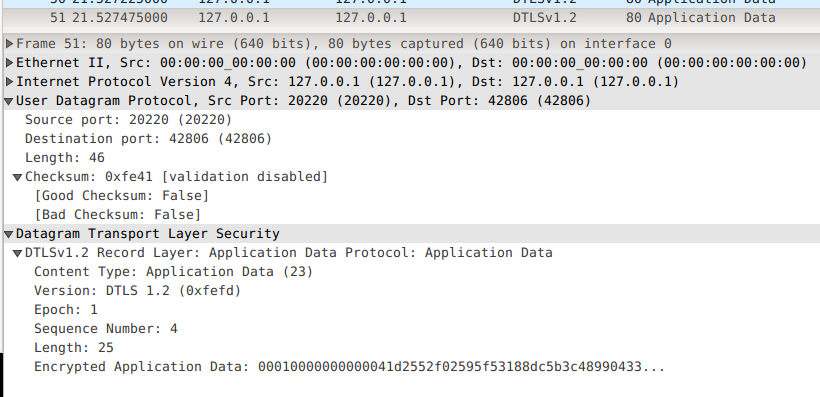
\includegraphics{./Pics/Sniffer.png}}
\caption{A Wireshark Screenshot}
\label{Fig: Sniffer}
\end{figure}

As we can see in  \Cref{Fig: Sniffer}, although the sniffer is not able to decrypt the packet, all headers until DTLS are indeed accessible.

\section{Motivation and Challenges}
The open nature of the development Internet of Things (IoT) demands more security and privacy measure. Unlike the stable and already-widely-deployed Internet, the structure of IoT network is still under a developing process; therefore it might be worthwhile to take into concern the security from an early stage.

One challenge in this project is the fundamental nature difference between network traffic and other physical side channel information. Many side channel attacks are aimed to recover secret key materials, such as DPA in \cite{DPA}, or Cache-timing Attack in \cite{Cache-Timing1} and \cite{Cache-Timing2}. 

Although it is not certain at this stage that whether there is a link between the value of cryptographic key chosen and packet headers, but intuitively they are more likely to be independent. The reason is that the cryptography primitives chosen should only affect the value of ciphertext which constitutes the payload; hence is expected to be transparent to the lower layer protocol headers. However, the timing information might still be exploited to recover the key material.

Different protocol suite result into different headers and hence different information. As a beginning for this project, we choose to study the traffic generated by a DTLS implementation called tinyDTLS\cite{tinyDTLS}. tinyDTLS is designed to be suitable for embedded systems and is one of the IoT candidates in the future.

%At current stage, we have developed a toy network application(\Cref{Chp: Toys}) to show that such potential of information leakage exists and demonstrated an attack method against the application. 

%The long term proposal of this project is to study what kind of information can be leaked through these unprotected meta data as well as any other kinds of  information an adversary can learn by simply capturing the network traffic. 
\chapter{Literature Review}

\section{Academic Publications}

\cite{Web1} demonstrated that this kind of  leakage indeed exists in some web applications. Firstly, different web page has different page sizes; thus the size can be exploited as a fingerprint to indicate which page the victim accessed. Secondly, on some pages where part of its content is generated dynamically, such as suggestions in a search box, the size of the dynamic content can again be used as a fingerprint and therefore reveal the victim's input which is supposed to be kept secret.

\cite{Web2} focuses on detecting leakage points of input in web applications. In this paper, a web applications is modelled as a finite state machine. Observable packet information, such as length and flags in a TCP header, are represented as a vector. A trace is then defined as a sequence of packet information. The leakage points are then measured by estimating the mutual information of  the input and each point in the trace. As an extension to mutual information analysis, \cite{DBLP:conf/csfw/AlvimCPS12} and \cite{DBLP:conf/csfw/ChothiaG11} provide methods to improve accuracy and performance of the test.

\cite{Web1} and \cite{Web2} together lay a foundation to this project. \cite{Web1} focuses more on the fact that information leakage through encrypted network traffic actually exists but the attacks it describes are relatively web-site specific, although this could be a feature in this subject. The mutual information test proposed in \cite{Web2} is a powerful tool to pinpoint the leakage points but it also suffers from a performance issue as it requires a huge amount of computation.

\cite{Danezis_trafficanalysis} and \cite{DBLP:journals/iacr/SchaubSHCJTHGR14} described two actual attacks using packet length. \cite{Danezis_trafficanalysis} uses packet length to fingerprint pages which contains potentially privacy information. \cite{DBLP:journals/iacr/SchaubSHCJTHGR14} attacks search keyword by profiling the size of response for each character typed in the search box, then matches the victim's traffic in a suffix tree built for the dictionary by a stochastic algorithm.

Packet length might be the most juicy target in packet analysis attacks. These are particularly efficient and requires only passive observation and not much effective countermeasures are proposed. However, the effectiveness of these attacks might be affected by divergence of packet lengths which can be seen common as a result of ads or other kinds of dynamic contents in web pages. One potential problem in \cite{DBLP:journals/iacr/SchaubSHCJTHGR14} is that the profiling step takes a long time due to the response time of search engine and the dictionary chosen also has a great impact on the efficiency and accuracy of attack. It might be worthy pointing out that most theoretical cryptographical research studies only secrecy of plaintexts with same length which is not the case in real world. I personally think that these attacks exploited a blind spot in theoretic study and have displayed the gap between theoretical world and practical world. Packet length is also the most studied side channel information in our experiment at this stage. (See \Cref{Chp: Progress To Date})

Compression ratio obtained by toggling the compress flag in some protocol can also be exploited to recover plaintext. The general idea of this kind of attack is described in \cite{DBLP:conf/fse/Kelsey02}. This attack requires the adversary being able to inject his guesses of plaintext into the uncompressed plaintext. The compression ratio will be relatively higher when the guess matches part of the plaintext and lower if it does not. \cite{CRIME} and \cite{BREACH} gave implementations against TLS and HTTPS in real scenarios respectively. \cite{DBLP:journals/iacr/AlawatugodaSB14a} proposed some countermeasures by disabling compression or inducing some length hiding mechanism.

At a first glance, the partial plaintext control assumption in \cite{DBLP:conf/fse/Kelsey02} seems to be weird, but \cite{BREACH} has demonstrated that such circumstances can be practically achieved by a phishing link. Further more, some crucial information can be attacked such as the session cookie which can then be used to hijack a https session, like on-line banking. As an impact of these attacks, the latest TLS standard has disabled the usage of compression. Nevertheless, when it comes to constrained environment where bandwidth becomes precious, a solution better than totally forbidden is desired. However, there is no compression in our current set up(see \Cref{Chp: Progress To Date}). This kind of attack is not considered at this stage.

\cite{DBLP:conf/eurocrypt/Vaudenay02} exploits the padding scheme of CBC mode\footnote{\url{http://en.wikipedia.org/wiki/Block_cipher_mode_of_operation\#Cipher_Block_Chaining_.28CBC.29}}
 to recover the plaintext. This attack is based on the fact that some SSL implementation returns different error messages on padding error and MAC failure. Since the padding verification is done after decryption but before MAC verification, the adversary can send to the server a partially modified ciphertext and recover the plaintext by different error messages. Although one countermeasure against this attack is to unify the error messages, \cite{DBLP:conf/sp/AlFardanP13} states that it is still possible to distinguish these errors by measuring the time difference induced by whether a MAC verification is performed.

The countermeasure against the attack in \cite{DBLP:conf/eurocrypt/Vaudenay02} has been adopted in many recent implementations by unifying the error message. The attack described \cite{DBLP:conf/sp/AlFardanP13} relies on the heartbeat being turned on and is very sensitive to network latency. Above that as stated in the paper that adding a idle time before respond can effectively prevent this attack. For a sensor network, the time resolution is expected to be higher due to the low processing power of devices. It is not clear at this stage whether this will raise the risk of this attack. However, the cipher suite adopted by our current experimental environment does not have any padding at all(see \Cref{Chp: Progress To Date}); hence this kind of attack is not being considered at this stage.

\section{Standard Specifications}
Another part of the related literatures are the RFC specifications\footnote{\url{http://www.ietf.org/rfc.html}}. As of this project, we tend to put our focus on the protocols from Network Layer to Secure Layer in \Cref{Tbl: OSI} as a consideration of generality. Therefore, the following documents can be regarded as main references of protocol specifications:

\begin{itemize}
\item{RFC 791\cite{rfc791}} is the IPv4 specification. IPv4 is the most widely deployed protocol today. Even though its successor IPv6 has been proposed for more than a decade, the replacing process is taking place very slowly. It is expected that IPv4 will remain its dominance over the next few years.

\item{RFC 2460\cite{rfc2460}} is the IPv6 specification. IPv6 is the successor of IPv4. It was published in 1998 due to the exhaustion of IPv4 address. Although kernels today usually support both IPv4 and IPv6, many applications are still based on IPv4. However, as a “next generation” network, many IoT manufacturers also have the trend of adopting IPv6 as their standard.

\item{RFC 6282\cite{rfc6282}} is the specification for 6lowPAN. 6lowPAN is a compression header format for IPv6. It is designed for applications over constrained environments such as sensor networks where the resources, like bandwidth, are very limited. Comparing to a standard IPv6 header, a 6lowPAN header omits some fields by setting them to a default value suitable for constrained environments and hence  saved some bandwidth as well as processing time.

\item{RFC 6347\cite{rfc6347}} is the DTLS specification. DTLS is the counterpart of TLS over UDP. Since DTLS relies on UDP instead of TCP therefore it is considered to be more lightweight but unreliable. Even though UDP is designed to be connectionless in order to reduce its overhead, DTLS additionally (comparing to TLS) implemented some connection-oriented feature such as sequence to remain functional.

\item{RFC 7252\cite{rfc7252}} is the specification document for Constrained Application Protocol, CoAP. CoAP is a general application protocol for constrained environment. It has a similar design to HTTP which has a Request-Respond model and supports methods including GET, POST, PUT and DELETE. CoAP is designed to be able to map to HTTP for interoperability purpose.
\end{itemize}
\chapter{Progress To Date}
\label{Chp: Progress To Date}

As a beginning of this project, our first step is to demonstrate that information leakage similar to those described in \cite{Web1} can be found when the underlying protocol is switched DTLS. The reason is that DTLS is more suitable to sensor networks comparing to TLS due to is relatively lightweight-ness. 

The basic idea is to build some toy applications which model typical sensor network traffic generated through DTLS. The information leakage of toy applications are intentionally crafted to emphasise their existence.

Even though both OpenSSL and GnuSSL have DTLS implemented with general features, we setted our experimental the less featured tinyDTLS\cite{tinyDTLS} due to its lightweight-ness, which is more suitable to sensor networks. However, the drawback is that only one cipher-suite, TLS\_ECDHE\_ECDSA\_WITH\_AES\_128\_CCM\_8\cite{rfc7251}, is available for the current version of tinyDTLS. This implies that there should be no padding scheme adopted and hence the length of plaintext and ciphertext are expected to have a linear relationship. Our experiments supported this conjecture such that:
\begin{equation} \label{Eq: Plaintext length}
l_D = 17 + l
\end{equation}
where $l$ is the length of plaintext and $l_D$ is the value in DTLS length field. According to the specifications the additional bytes is supposed to be purely a resulted of the appending MAC even though $17$ bytes is a value unlikely to be. This problem is still under investigating.

All experiments are done with only two processes, a server and a client referred as SERVER and CLIENT, on a same linux host connected through local-link. The protocol suite we adopted is [IPv4 or IPv6] + UDP + DTLS. The modelled adversary is simply a passive eavesdropper.

So far we have built up two toy applications, \textbf{Odd or Even} and \textbf{Leaky Coffee}, which will be explained in the next sessions alongside with corresponding traffic analysis.

\section{Odd or Even} \label{Sec: Odd or Even}
\textbf{Odd or Even} is a simple toy application designed  to demonstrate the fundamental idea of encrypted traffic analysis.

\subsection{Application Description}

\begin{figure}[H] 
\centering
\resizebox{8cm}{!}
{% Graphic for TeX using PGF
% Title: /home/yy12135/MyGit/tinyDTLS-Traffic-Analysis/Writings/First-year-review_20150422/Pics/OddOrEven.dia
% Creator: Dia v0.97.2
% CreationDate: Mon Mar  2 17:12:59 2015
% For: yy12135
% \usepackage{tikz}
% The following commands are not supported in PSTricks at present
% We define them conditionally, so when they are implemented,
% this pgf file will use them.
\ifx\du\undefined
  \newlength{\du}
\fi
\setlength{\du}{15\unitlength}
\begin{tikzpicture}
\pgftransformxscale{1.000000}
\pgftransformyscale{-1.000000}
\definecolor{dialinecolor}{rgb}{0.000000, 0.000000, 0.000000}
\pgfsetstrokecolor{dialinecolor}
\definecolor{dialinecolor}{rgb}{1.000000, 1.000000, 1.000000}
\pgfsetfillcolor{dialinecolor}
% setfont left to latex
\definecolor{dialinecolor}{rgb}{0.000000, 0.000000, 0.000000}
\pgfsetstrokecolor{dialinecolor}
\node[anchor=west] at (11.000000\du,9.000000\du){};
\definecolor{dialinecolor}{rgb}{1.000000, 1.000000, 1.000000}
\pgfsetfillcolor{dialinecolor}
\pgfpathellipse{\pgfpoint{31.003315\du}{10.006491\du}}{\pgfpoint{1.831366\du}{0\du}}{\pgfpoint{0\du}{1.837164\du}}
\pgfusepath{fill}
\pgfsetlinewidth{0.100000\du}
\pgfsetdash{}{0pt}
\pgfsetdash{}{0pt}
\pgfsetmiterjoin
\definecolor{dialinecolor}{rgb}{0.000000, 0.000000, 0.000000}
\pgfsetstrokecolor{dialinecolor}
\pgfpathellipse{\pgfpoint{31.003315\du}{10.006491\du}}{\pgfpoint{1.831366\du}{0\du}}{\pgfpoint{0\du}{1.837164\du}}
\pgfusepath{stroke}
% setfont left to latex
\definecolor{dialinecolor}{rgb}{0.000000, 0.000000, 0.000000}
\pgfsetstrokecolor{dialinecolor}
\node at (31.003315\du,10.201491\du){SERVER};
\pgfsetlinewidth{0.100000\du}
\pgfsetdash{}{0pt}
\pgfsetdash{}{0pt}
\pgfsetbuttcap
{
\definecolor{dialinecolor}{rgb}{0.000000, 0.000000, 0.000000}
\pgfsetfillcolor{dialinecolor}
% was here!!!
\pgfsetarrowsend{stealth}
\definecolor{dialinecolor}{rgb}{0.000000, 0.000000, 0.000000}
\pgfsetstrokecolor{dialinecolor}
\draw (31.002868\du,11.893189\du)--(31.000000\du,24.000000\du);
}
\pgfsetlinewidth{0.100000\du}
\pgfsetdash{}{0pt}
\pgfsetdash{}{0pt}
\pgfsetbuttcap
{
\definecolor{dialinecolor}{rgb}{0.000000, 0.000000, 0.000000}
\pgfsetfillcolor{dialinecolor}
% was here!!!
\pgfsetarrowsend{to}
\definecolor{dialinecolor}{rgb}{0.000000, 0.000000, 0.000000}
\pgfsetstrokecolor{dialinecolor}
\draw (15.036382\du,13.528274\du)--(31.002048\du,15.352278\du);
}
\pgfsetlinewidth{0.100000\du}
\pgfsetdash{}{0pt}
\pgfsetdash{}{0pt}
\pgfsetbuttcap
{
\definecolor{dialinecolor}{rgb}{0.000000, 0.000000, 0.000000}
\pgfsetfillcolor{dialinecolor}
% was here!!!
\pgfsetarrowsend{to}
\definecolor{dialinecolor}{rgb}{0.000000, 0.000000, 0.000000}
\pgfsetstrokecolor{dialinecolor}
\draw (31.001229\du,18.811367\du)--(15.012127\du,20.509425\du);
}
\definecolor{dialinecolor}{rgb}{1.000000, 1.000000, 1.000000}
\pgfsetfillcolor{dialinecolor}
\pgfpathellipse{\pgfpoint{15.048531\du}{10.031365\du}}{\pgfpoint{1.729717\du}{0\du}}{\pgfpoint{0\du}{1.701399\du}}
\pgfusepath{fill}
\pgfsetlinewidth{0.100000\du}
\pgfsetdash{}{0pt}
\pgfsetdash{}{0pt}
\pgfsetmiterjoin
\definecolor{dialinecolor}{rgb}{0.000000, 0.000000, 0.000000}
\pgfsetstrokecolor{dialinecolor}
\pgfpathellipse{\pgfpoint{15.048531\du}{10.031365\du}}{\pgfpoint{1.729717\du}{0\du}}{\pgfpoint{0\du}{1.701399\du}}
\pgfusepath{stroke}
% setfont left to latex
\definecolor{dialinecolor}{rgb}{0.000000, 0.000000, 0.000000}
\pgfsetstrokecolor{dialinecolor}
\node at (15.048531\du,10.226365\du){CLIENT};
\pgfsetlinewidth{0.100000\du}
\pgfsetdash{}{0pt}
\pgfsetdash{}{0pt}
\pgfsetbuttcap
{
\definecolor{dialinecolor}{rgb}{0.000000, 0.000000, 0.000000}
\pgfsetfillcolor{dialinecolor}
% was here!!!
\pgfsetarrowsend{stealth}
\definecolor{dialinecolor}{rgb}{0.000000, 0.000000, 0.000000}
\pgfsetstrokecolor{dialinecolor}
\draw (15.042445\du,11.782986\du)--(15.000000\du,24.000000\du);
}
\pgfsetlinewidth{0.100000\du}
\pgfsetdash{}{0pt}
\pgfsetdash{}{0pt}
\pgfsetbuttcap
\pgfsetmiterjoin
\pgfsetlinewidth{0.100000\du}
\pgfsetbuttcap
\pgfsetmiterjoin
\pgfsetdash{}{0pt}
\definecolor{dialinecolor}{rgb}{1.000000, 1.000000, 1.000000}
\pgfsetfillcolor{dialinecolor}
\pgfpathmoveto{\pgfpoint{20.833333\du}{13.000000\du}}
\pgfpathlineto{\pgfpoint{24.166667\du}{13.000000\du}}
\pgfpathcurveto{\pgfpoint{24.626904\du}{13.000000\du}}{\pgfpoint{25.000000\du}{13.447715\du}}{\pgfpoint{25.000000\du}{14.000000\du}}
\pgfpathcurveto{\pgfpoint{25.000000\du}{14.552285\du}}{\pgfpoint{24.626904\du}{15.000000\du}}{\pgfpoint{24.166667\du}{15.000000\du}}
\pgfpathlineto{\pgfpoint{20.833333\du}{15.000000\du}}
\pgfpathcurveto{\pgfpoint{20.373096\du}{15.000000\du}}{\pgfpoint{20.000000\du}{14.552285\du}}{\pgfpoint{20.000000\du}{14.000000\du}}
\pgfpathcurveto{\pgfpoint{20.000000\du}{13.447715\du}}{\pgfpoint{20.373096\du}{13.000000\du}}{\pgfpoint{20.833333\du}{13.000000\du}}
\pgfusepath{fill}
\definecolor{dialinecolor}{rgb}{0.000000, 0.000000, 0.000000}
\pgfsetstrokecolor{dialinecolor}
\pgfpathmoveto{\pgfpoint{20.833333\du}{13.000000\du}}
\pgfpathlineto{\pgfpoint{24.166667\du}{13.000000\du}}
\pgfpathcurveto{\pgfpoint{24.626904\du}{13.000000\du}}{\pgfpoint{25.000000\du}{13.447715\du}}{\pgfpoint{25.000000\du}{14.000000\du}}
\pgfpathcurveto{\pgfpoint{25.000000\du}{14.552285\du}}{\pgfpoint{24.626904\du}{15.000000\du}}{\pgfpoint{24.166667\du}{15.000000\du}}
\pgfpathlineto{\pgfpoint{20.833333\du}{15.000000\du}}
\pgfpathcurveto{\pgfpoint{20.373096\du}{15.000000\du}}{\pgfpoint{20.000000\du}{14.552285\du}}{\pgfpoint{20.000000\du}{14.000000\du}}
\pgfpathcurveto{\pgfpoint{20.000000\du}{13.447715\du}}{\pgfpoint{20.373096\du}{13.000000\du}}{\pgfpoint{20.833333\du}{13.000000\du}}
\pgfusepath{stroke}
% setfont left to latex
\definecolor{dialinecolor}{rgb}{0.000000, 0.000000, 0.000000}
\pgfsetstrokecolor{dialinecolor}
\node at (22.500000\du,14.200000\du){32bit R};
\pgfsetlinewidth{0.100000\du}
\pgfsetdash{}{0pt}
\pgfsetdash{}{0pt}
\pgfsetbuttcap
\pgfsetmiterjoin
\pgfsetlinewidth{0.100000\du}
\pgfsetbuttcap
\pgfsetmiterjoin
\pgfsetdash{}{0pt}
\definecolor{dialinecolor}{rgb}{1.000000, 1.000000, 1.000000}
\pgfsetfillcolor{dialinecolor}
\pgfpathmoveto{\pgfpoint{20.228125\du}{18.000000\du}}
\pgfpathlineto{\pgfpoint{25.140625\du}{18.000000\du}}
\pgfpathcurveto{\pgfpoint{25.818900\du}{18.000000\du}}{\pgfpoint{26.368750\du}{18.447715\du}}{\pgfpoint{26.368750\du}{19.000000\du}}
\pgfpathcurveto{\pgfpoint{26.368750\du}{19.552285\du}}{\pgfpoint{25.818900\du}{20.000000\du}}{\pgfpoint{25.140625\du}{20.000000\du}}
\pgfpathlineto{\pgfpoint{20.228125\du}{20.000000\du}}
\pgfpathcurveto{\pgfpoint{19.549850\du}{20.000000\du}}{\pgfpoint{19.000000\du}{19.552285\du}}{\pgfpoint{19.000000\du}{19.000000\du}}
\pgfpathcurveto{\pgfpoint{19.000000\du}{18.447715\du}}{\pgfpoint{19.549850\du}{18.000000\du}}{\pgfpoint{20.228125\du}{18.000000\du}}
\pgfusepath{fill}
\definecolor{dialinecolor}{rgb}{0.000000, 0.000000, 0.000000}
\pgfsetstrokecolor{dialinecolor}
\pgfpathmoveto{\pgfpoint{20.228125\du}{18.000000\du}}
\pgfpathlineto{\pgfpoint{25.140625\du}{18.000000\du}}
\pgfpathcurveto{\pgfpoint{25.818900\du}{18.000000\du}}{\pgfpoint{26.368750\du}{18.447715\du}}{\pgfpoint{26.368750\du}{19.000000\du}}
\pgfpathcurveto{\pgfpoint{26.368750\du}{19.552285\du}}{\pgfpoint{25.818900\du}{20.000000\du}}{\pgfpoint{25.140625\du}{20.000000\du}}
\pgfpathlineto{\pgfpoint{20.228125\du}{20.000000\du}}
\pgfpathcurveto{\pgfpoint{19.549850\du}{20.000000\du}}{\pgfpoint{19.000000\du}{19.552285\du}}{\pgfpoint{19.000000\du}{19.000000\du}}
\pgfpathcurveto{\pgfpoint{19.000000\du}{18.447715\du}}{\pgfpoint{19.549850\du}{18.000000\du}}{\pgfpoint{20.228125\du}{18.000000\du}}
\pgfusepath{stroke}
% setfont left to latex
\definecolor{dialinecolor}{rgb}{0.000000, 0.000000, 0.000000}
\pgfsetstrokecolor{dialinecolor}
\node at (22.684375\du,19.200000\du){"ODD"/"EVEN"};
\end{tikzpicture}
}
\caption{Description of an Odd-or-Even session}
\label{Fig: Odd or Even}
\end{figure}

CLIENT randomly generates a 32-bit unsigned integer R and sends it to SERVER in binary. SERVER replies with a string “ODD'' or “EVEN” according to the value of the 32-bit $R$(\Cref{Fig: Odd or Even}).

\subsection{Analysis}
We run the application for multiple times and collected the packets it generated. As we have expected, “ODD” packets are $1$ byte shorter than “EVEN” packets which implies that an eavesdropping adversary can learn what has been sent from SERVER to CLIENT simply by looking at the packets length. However, no obvious leakage has been found in other fields of the packets.

%For every \textbf{Odd-or-Even} session, 
%
%Packets from CLIENT to SERVER:
%
%All fields for every packet are the same, except:
%1. Encrypted Application Data field in DTLS layer.
%2. Sequence Number increased by 1 every packet.
%3. Checksum in UDP layer.
%
%Packets from SERVER to CLIENT:
%
%All fields are the same for every packet except:
%1. Encrypted Application Data field in DTLS layer.
%2. Sequence Number increased by 1 every packet.
%3. Checksum in UDP layer.
%4. Length field in both DTLS layer and UDP layer. The values are always (20,41) respectively when data is "Odd" and (21,42) when data is "Even".
%
%Therefore in this application, given pre-knowledge that server responds with either "Odd" or "Even", the length field in both DTLS layer and UDP layer can directly leak the plaintext. 

\section{Leaky Coffee}
\label{Sec: Leaky Coffee}

\subsection{Application Description}
\textbf{Leaky Coffee} simulates a more complicated scenario where the CLIENT sends a coffee order (in string) to SERVER. SERVER echoes the order appended by some flavour (in string). CLIENT compares the amount of given flavour to an internally generated random requirement and asks SERVER again for more additive if it is insufficient.

\begin{figure}[H]
\centering
\resizebox{12cm}{!}
{% Graphic for TeX using PGF
% Title: /home/yy12135/Google Drive/Writings/First-year-review_20150422/Pics/LeakyCoffee.dia
% Creator: Dia v0.97.2
% CreationDate: Tue Mar  3 14:05:39 2015
% For: yy12135
% \usepackage{tikz}
% The following commands are not supported in PSTricks at present
% We define them conditionally, so when they are implemented,
% this pgf file will use them.
\ifx\du\undefined
  \newlength{\du}
\fi
\setlength{\du}{15\unitlength}
\begin{tikzpicture}
\pgftransformxscale{1.000000}
\pgftransformyscale{-1.000000}
\definecolor{dialinecolor}{rgb}{0.000000, 0.000000, 0.000000}
\pgfsetstrokecolor{dialinecolor}
\definecolor{dialinecolor}{rgb}{1.000000, 1.000000, 1.000000}
\pgfsetfillcolor{dialinecolor}
\definecolor{dialinecolor}{rgb}{1.000000, 1.000000, 1.000000}
\pgfsetfillcolor{dialinecolor}
\pgfpathellipse{\pgfpoint{10.000000\du}{11.000000\du}}{\pgfpoint{1.723870\du}{0\du}}{\pgfpoint{0\du}{1.723870\du}}
\pgfusepath{fill}
\pgfsetlinewidth{0.100000\du}
\pgfsetdash{}{0pt}
\pgfsetdash{}{0pt}
\pgfsetmiterjoin
\definecolor{dialinecolor}{rgb}{0.000000, 0.000000, 0.000000}
\pgfsetstrokecolor{dialinecolor}
\pgfpathellipse{\pgfpoint{10.000000\du}{11.000000\du}}{\pgfpoint{1.723870\du}{0\du}}{\pgfpoint{0\du}{1.723870\du}}
\pgfusepath{stroke}
% setfont left to latex
\definecolor{dialinecolor}{rgb}{0.000000, 0.000000, 0.000000}
\pgfsetstrokecolor{dialinecolor}
\node at (10.000000\du,11.195000\du){CLIENT};
% setfont left to latex
\definecolor{dialinecolor}{rgb}{0.000000, 0.000000, 0.000000}
\pgfsetstrokecolor{dialinecolor}
\node[anchor=west] at (10.000000\du,11.000000\du){};
\definecolor{dialinecolor}{rgb}{1.000000, 1.000000, 1.000000}
\pgfsetfillcolor{dialinecolor}
\pgfpathellipse{\pgfpoint{25.008494\du}{10.996126\du}}{\pgfpoint{1.836494\du}{0\du}}{\pgfpoint{0\du}{1.813886\du}}
\pgfusepath{fill}
\pgfsetlinewidth{0.100000\du}
\pgfsetdash{}{0pt}
\pgfsetdash{}{0pt}
\pgfsetmiterjoin
\definecolor{dialinecolor}{rgb}{0.000000, 0.000000, 0.000000}
\pgfsetstrokecolor{dialinecolor}
\pgfpathellipse{\pgfpoint{25.008494\du}{10.996126\du}}{\pgfpoint{1.836494\du}{0\du}}{\pgfpoint{0\du}{1.813886\du}}
\pgfusepath{stroke}
% setfont left to latex
\definecolor{dialinecolor}{rgb}{0.000000, 0.000000, 0.000000}
\pgfsetstrokecolor{dialinecolor}
\node at (25.008494\du,11.191126\du){SERVER};
\pgfsetlinewidth{0.100000\du}
\pgfsetdash{}{0pt}
\pgfsetdash{}{0pt}
\pgfsetbuttcap
{
\definecolor{dialinecolor}{rgb}{0.000000, 0.000000, 0.000000}
\pgfsetfillcolor{dialinecolor}
% was here!!!
\pgfsetarrowsend{to}
\definecolor{dialinecolor}{rgb}{0.000000, 0.000000, 0.000000}
\pgfsetstrokecolor{dialinecolor}
\draw (10.000000\du,12.774002\du)--(10.000000\du,40.000000\du);
}
\pgfsetlinewidth{0.100000\du}
\pgfsetdash{}{0pt}
\pgfsetdash{}{0pt}
\pgfsetbuttcap
{
\definecolor{dialinecolor}{rgb}{0.000000, 0.000000, 0.000000}
\pgfsetfillcolor{dialinecolor}
% was here!!!
\pgfsetarrowsend{to}
\definecolor{dialinecolor}{rgb}{0.000000, 0.000000, 0.000000}
\pgfsetstrokecolor{dialinecolor}
\draw (25.007949\du,12.859321\du)--(25.000000\du,40.000000\du);
}
\pgfsetlinewidth{0.100000\du}
\pgfsetdash{}{0pt}
\pgfsetdash{}{0pt}
\pgfsetbuttcap
{
\definecolor{dialinecolor}{rgb}{0.000000, 0.000000, 0.000000}
\pgfsetfillcolor{dialinecolor}
% was here!!!
\pgfsetarrowsend{to}
\definecolor{dialinecolor}{rgb}{0.000000, 0.000000, 0.000000}
\pgfsetstrokecolor{dialinecolor}
\draw (10.000000\du,15.799100\du)--(25.006200\du,18.890600\du);
}
\pgfsetlinewidth{0.100000\du}
\pgfsetdash{}{0pt}
\pgfsetdash{}{0pt}
\pgfsetbuttcap
{
\definecolor{dialinecolor}{rgb}{0.000000, 0.000000, 0.000000}
\pgfsetfillcolor{dialinecolor}
% was here!!!
\pgfsetarrowsend{to}
\definecolor{dialinecolor}{rgb}{0.000000, 0.000000, 0.000000}
\pgfsetstrokecolor{dialinecolor}
\draw (25.005300\du,21.906200\du)--(10.000000\du,24.874400\du);
}
\pgfsetlinewidth{0.100000\du}
\pgfsetdash{}{0pt}
\pgfsetdash{}{0pt}
\pgfsetbuttcap
\pgfsetmiterjoin
\pgfsetlinewidth{0.100000\du}
\pgfsetbuttcap
\pgfsetmiterjoin
\pgfsetdash{}{0pt}
\definecolor{dialinecolor}{rgb}{1.000000, 1.000000, 1.000000}
\pgfsetfillcolor{dialinecolor}
\pgfpathmoveto{\pgfpoint{13.558175\du}{16.000000\du}}
\pgfpathlineto{\pgfpoint{19.625675\du}{16.000000\du}}
\pgfpathcurveto{\pgfpoint{20.463422\du}{16.000000\du}}{\pgfpoint{21.142550\du}{16.447715\du}}{\pgfpoint{21.142550\du}{17.000000\du}}
\pgfpathcurveto{\pgfpoint{21.142550\du}{17.552285\du}}{\pgfpoint{20.463422\du}{18.000000\du}}{\pgfpoint{19.625675\du}{18.000000\du}}
\pgfpathlineto{\pgfpoint{13.558175\du}{18.000000\du}}
\pgfpathcurveto{\pgfpoint{12.720428\du}{18.000000\du}}{\pgfpoint{12.041300\du}{17.552285\du}}{\pgfpoint{12.041300\du}{17.000000\du}}
\pgfpathcurveto{\pgfpoint{12.041300\du}{16.447715\du}}{\pgfpoint{12.720428\du}{16.000000\du}}{\pgfpoint{13.558175\du}{16.000000\du}}
\pgfusepath{fill}
\definecolor{dialinecolor}{rgb}{0.000000, 0.000000, 0.000000}
\pgfsetstrokecolor{dialinecolor}
\pgfpathmoveto{\pgfpoint{13.558175\du}{16.000000\du}}
\pgfpathlineto{\pgfpoint{19.625675\du}{16.000000\du}}
\pgfpathcurveto{\pgfpoint{20.463422\du}{16.000000\du}}{\pgfpoint{21.142550\du}{16.447715\du}}{\pgfpoint{21.142550\du}{17.000000\du}}
\pgfpathcurveto{\pgfpoint{21.142550\du}{17.552285\du}}{\pgfpoint{20.463422\du}{18.000000\du}}{\pgfpoint{19.625675\du}{18.000000\du}}
\pgfpathlineto{\pgfpoint{13.558175\du}{18.000000\du}}
\pgfpathcurveto{\pgfpoint{12.720428\du}{18.000000\du}}{\pgfpoint{12.041300\du}{17.552285\du}}{\pgfpoint{12.041300\du}{17.000000\du}}
\pgfpathcurveto{\pgfpoint{12.041300\du}{16.447715\du}}{\pgfpoint{12.720428\du}{16.000000\du}}{\pgfpoint{13.558175\du}{16.000000\du}}
\pgfusepath{stroke}
% setfont left to latex
\definecolor{dialinecolor}{rgb}{0.000000, 0.000000, 0.000000}
\pgfsetstrokecolor{dialinecolor}
\node at (16.591925\du,17.200000\du){\textbf{1}. $Order$};
\pgfsetlinewidth{0.100000\du}
\pgfsetdash{}{0pt}
\pgfsetdash{}{0pt}
\pgfsetbuttcap
\pgfsetmiterjoin
\pgfsetlinewidth{0.100000\du}
\pgfsetbuttcap
\pgfsetmiterjoin
\pgfsetdash{}{0pt}
\definecolor{dialinecolor}{rgb}{1.000000, 1.000000, 1.000000}
\pgfsetfillcolor{dialinecolor}
\pgfpathmoveto{\pgfpoint{12.990000\du}{22.000000\du}}
\pgfpathlineto{\pgfpoint{20.950000\du}{22.000000\du}}
\pgfpathcurveto{\pgfpoint{22.049047\du}{22.000000\du}}{\pgfpoint{22.940000\du}{22.447715\du}}{\pgfpoint{22.940000\du}{23.000000\du}}
\pgfpathcurveto{\pgfpoint{22.940000\du}{23.552285\du}}{\pgfpoint{22.049047\du}{24.000000\du}}{\pgfpoint{20.950000\du}{24.000000\du}}
\pgfpathlineto{\pgfpoint{12.990000\du}{24.000000\du}}
\pgfpathcurveto{\pgfpoint{11.890953\du}{24.000000\du}}{\pgfpoint{11.000000\du}{23.552285\du}}{\pgfpoint{11.000000\du}{23.000000\du}}
\pgfpathcurveto{\pgfpoint{11.000000\du}{22.447715\du}}{\pgfpoint{11.890953\du}{22.000000\du}}{\pgfpoint{12.990000\du}{22.000000\du}}
\pgfusepath{fill}
\definecolor{dialinecolor}{rgb}{0.000000, 0.000000, 0.000000}
\pgfsetstrokecolor{dialinecolor}
\pgfpathmoveto{\pgfpoint{12.990000\du}{22.000000\du}}
\pgfpathlineto{\pgfpoint{20.950000\du}{22.000000\du}}
\pgfpathcurveto{\pgfpoint{22.049047\du}{22.000000\du}}{\pgfpoint{22.940000\du}{22.447715\du}}{\pgfpoint{22.940000\du}{23.000000\du}}
\pgfpathcurveto{\pgfpoint{22.940000\du}{23.552285\du}}{\pgfpoint{22.049047\du}{24.000000\du}}{\pgfpoint{20.950000\du}{24.000000\du}}
\pgfpathlineto{\pgfpoint{12.990000\du}{24.000000\du}}
\pgfpathcurveto{\pgfpoint{11.890953\du}{24.000000\du}}{\pgfpoint{11.000000\du}{23.552285\du}}{\pgfpoint{11.000000\du}{23.000000\du}}
\pgfpathcurveto{\pgfpoint{11.000000\du}{22.447715\du}}{\pgfpoint{11.890953\du}{22.000000\du}}{\pgfpoint{12.990000\du}{22.000000\du}}
\pgfusepath{stroke}
% setfont left to latex
\definecolor{dialinecolor}{rgb}{0.000000, 0.000000, 0.000000}
\pgfsetstrokecolor{dialinecolor}
\node at (16.970000\du,23.200000\du){\textbf{2}.$Coffee$};
\pgfsetlinewidth{0.100000\du}
\pgfsetdash{{1.000000\du}{1.000000\du}}{0\du}
\pgfsetdash{{1.000000\du}{1.000000\du}}{0\du}
\pgfsetbuttcap
{
\definecolor{dialinecolor}{rgb}{0.000000, 0.000000, 0.000000}
\pgfsetfillcolor{dialinecolor}
% was here!!!
\definecolor{dialinecolor}{rgb}{0.000000, 0.000000, 0.000000}
\pgfsetstrokecolor{dialinecolor}
\draw (9.010000\du,25.950000\du)--(36.000000\du,26.000000\du);
}
\definecolor{dialinecolor}{rgb}{1.000000, 1.000000, 1.000000}
\pgfsetfillcolor{dialinecolor}
\fill (0.000000\du,25.000000\du)--(0.000000\du,26.900000\du)--(9.010000\du,26.900000\du)--(9.010000\du,25.000000\du)--cycle;
\pgfsetlinewidth{0.100000\du}
\pgfsetdash{}{0pt}
\pgfsetdash{}{0pt}
\pgfsetmiterjoin
\definecolor{dialinecolor}{rgb}{0.000000, 0.000000, 0.000000}
\pgfsetstrokecolor{dialinecolor}
\draw (0.000000\du,25.000000\du)--(0.000000\du,26.900000\du)--(9.010000\du,26.900000\du)--(9.010000\du,25.000000\du)--cycle;
% setfont left to latex
\definecolor{dialinecolor}{rgb}{0.000000, 0.000000, 0.000000}
\pgfsetstrokecolor{dialinecolor}
\node at (4.505000\du,26.145000\du){If $Flavour$ is not enough};
\pgfsetlinewidth{0.100000\du}
\pgfsetdash{}{0pt}
\pgfsetdash{}{0pt}
\pgfsetbuttcap
{
\definecolor{dialinecolor}{rgb}{0.000000, 0.000000, 0.000000}
\pgfsetfillcolor{dialinecolor}
% was here!!!
\pgfsetarrowsend{to}
\definecolor{dialinecolor}{rgb}{0.000000, 0.000000, 0.000000}
\pgfsetstrokecolor{dialinecolor}
\draw (10.000000\du,27.899600\du)--(25.002700\du,30.953100\du);
}
\pgfsetlinewidth{0.100000\du}
\pgfsetdash{}{0pt}
\pgfsetdash{}{0pt}
\pgfsetbuttcap
\pgfsetmiterjoin
\pgfsetlinewidth{0.100000\du}
\pgfsetbuttcap
\pgfsetmiterjoin
\pgfsetdash{}{0pt}
\definecolor{dialinecolor}{rgb}{1.000000, 1.000000, 1.000000}
\pgfsetfillcolor{dialinecolor}
\pgfpathmoveto{\pgfpoint{14.065625\du}{28.000000\du}}
\pgfpathlineto{\pgfpoint{20.158125\du}{28.000000\du}}
\pgfpathcurveto{\pgfpoint{20.999324\du}{28.000000\du}}{\pgfpoint{21.681250\du}{28.447715\du}}{\pgfpoint{21.681250\du}{29.000000\du}}
\pgfpathcurveto{\pgfpoint{21.681250\du}{29.552285\du}}{\pgfpoint{20.999324\du}{30.000000\du}}{\pgfpoint{20.158125\du}{30.000000\du}}
\pgfpathlineto{\pgfpoint{14.065625\du}{30.000000\du}}
\pgfpathcurveto{\pgfpoint{13.224426\du}{30.000000\du}}{\pgfpoint{12.542500\du}{29.552285\du}}{\pgfpoint{12.542500\du}{29.000000\du}}
\pgfpathcurveto{\pgfpoint{12.542500\du}{28.447715\du}}{\pgfpoint{13.224426\du}{28.000000\du}}{\pgfpoint{14.065625\du}{28.000000\du}}
\pgfusepath{fill}
\definecolor{dialinecolor}{rgb}{0.000000, 0.000000, 0.000000}
\pgfsetstrokecolor{dialinecolor}
\pgfpathmoveto{\pgfpoint{14.065625\du}{28.000000\du}}
\pgfpathlineto{\pgfpoint{20.158125\du}{28.000000\du}}
\pgfpathcurveto{\pgfpoint{20.999324\du}{28.000000\du}}{\pgfpoint{21.681250\du}{28.447715\du}}{\pgfpoint{21.681250\du}{29.000000\du}}
\pgfpathcurveto{\pgfpoint{21.681250\du}{29.552285\du}}{\pgfpoint{20.999324\du}{30.000000\du}}{\pgfpoint{20.158125\du}{30.000000\du}}
\pgfpathlineto{\pgfpoint{14.065625\du}{30.000000\du}}
\pgfpathcurveto{\pgfpoint{13.224426\du}{30.000000\du}}{\pgfpoint{12.542500\du}{29.552285\du}}{\pgfpoint{12.542500\du}{29.000000\du}}
\pgfpathcurveto{\pgfpoint{12.542500\du}{28.447715\du}}{\pgfpoint{13.224426\du}{28.000000\du}}{\pgfpoint{14.065625\du}{28.000000\du}}
\pgfusepath{stroke}
% setfont left to latex
\definecolor{dialinecolor}{rgb}{0.000000, 0.000000, 0.000000}
\pgfsetstrokecolor{dialinecolor}
\node at (17.111875\du,29.200000\du){\textbf{3}.$FlavourRequest$};
\pgfsetlinewidth{0.100000\du}
\pgfsetdash{{1.000000\du}{1.000000\du}}{0\du}
\pgfsetdash{{1.000000\du}{1.000000\du}}{0\du}
\pgfsetbuttcap
{
\definecolor{dialinecolor}{rgb}{0.000000, 0.000000, 0.000000}
\pgfsetfillcolor{dialinecolor}
% was here!!!
\definecolor{dialinecolor}{rgb}{0.000000, 0.000000, 0.000000}
\pgfsetstrokecolor{dialinecolor}
\draw (1.000000\du,38.000000\du)--(36.000000\du,38.000000\du);
}
\pgfsetlinewidth{0.100000\du}
\pgfsetdash{}{0pt}
\pgfsetdash{}{0pt}
\pgfsetbuttcap
{
\definecolor{dialinecolor}{rgb}{0.000000, 0.000000, 0.000000}
\pgfsetfillcolor{dialinecolor}
% was here!!!
\pgfsetarrowsend{to}
\definecolor{dialinecolor}{rgb}{0.000000, 0.000000, 0.000000}
\pgfsetstrokecolor{dialinecolor}
\draw (25.001800\du,33.968700\du)--(10.000000\du,36.974900\du);
}
\pgfsetlinewidth{0.100000\du}
\pgfsetdash{}{0pt}
\pgfsetdash{}{0pt}
\pgfsetbuttcap
\pgfsetmiterjoin
\pgfsetlinewidth{0.100000\du}
\pgfsetbuttcap
\pgfsetmiterjoin
\pgfsetdash{}{0pt}
\definecolor{dialinecolor}{rgb}{1.000000, 1.000000, 1.000000}
\pgfsetfillcolor{dialinecolor}
\pgfpathmoveto{\pgfpoint{13.779375\du}{34.000000\du}}
\pgfpathlineto{\pgfpoint{20.236875\du}{34.000000\du}}
\pgfpathcurveto{\pgfpoint{21.128470\du}{34.000000\du}}{\pgfpoint{21.851250\du}{34.447715\du}}{\pgfpoint{21.851250\du}{35.000000\du}}
\pgfpathcurveto{\pgfpoint{21.851250\du}{35.552285\du}}{\pgfpoint{21.128470\du}{36.000000\du}}{\pgfpoint{20.236875\du}{36.000000\du}}
\pgfpathlineto{\pgfpoint{13.779375\du}{36.000000\du}}
\pgfpathcurveto{\pgfpoint{12.887780\du}{36.000000\du}}{\pgfpoint{12.165000\du}{35.552285\du}}{\pgfpoint{12.165000\du}{35.000000\du}}
\pgfpathcurveto{\pgfpoint{12.165000\du}{34.447715\du}}{\pgfpoint{12.887780\du}{34.000000\du}}{\pgfpoint{13.779375\du}{34.000000\du}}
\pgfusepath{fill}
\definecolor{dialinecolor}{rgb}{0.000000, 0.000000, 0.000000}
\pgfsetstrokecolor{dialinecolor}
\pgfpathmoveto{\pgfpoint{13.779375\du}{34.000000\du}}
\pgfpathlineto{\pgfpoint{20.236875\du}{34.000000\du}}
\pgfpathcurveto{\pgfpoint{21.128470\du}{34.000000\du}}{\pgfpoint{21.851250\du}{34.447715\du}}{\pgfpoint{21.851250\du}{35.000000\du}}
\pgfpathcurveto{\pgfpoint{21.851250\du}{35.552285\du}}{\pgfpoint{21.128470\du}{36.000000\du}}{\pgfpoint{20.236875\du}{36.000000\du}}
\pgfpathlineto{\pgfpoint{13.779375\du}{36.000000\du}}
\pgfpathcurveto{\pgfpoint{12.887780\du}{36.000000\du}}{\pgfpoint{12.165000\du}{35.552285\du}}{\pgfpoint{12.165000\du}{35.000000\du}}
\pgfpathcurveto{\pgfpoint{12.165000\du}{34.447715\du}}{\pgfpoint{12.887780\du}{34.000000\du}}{\pgfpoint{13.779375\du}{34.000000\du}}
\pgfusepath{stroke}
% setfont left to latex
\definecolor{dialinecolor}{rgb}{0.000000, 0.000000, 0.000000}
\pgfsetstrokecolor{dialinecolor}
\node at (17.008125\du,35.200000\du){\textbf{4}.$FlavourResponse$};
\pgfsetlinewidth{0.100000\du}
\pgfsetdash{{1.000000\du}{1.000000\du}}{0\du}
\pgfsetdash{{1.000000\du}{1.000000\du}}{0\du}
\pgfsetbuttcap
{
\definecolor{dialinecolor}{rgb}{0.000000, 0.000000, 0.000000}
\pgfsetfillcolor{dialinecolor}
% was here!!!
\pgfsetarrowsstart{to}
\pgfsetarrowsend{to}
\definecolor{dialinecolor}{rgb}{0.000000, 0.000000, 0.000000}
\pgfsetstrokecolor{dialinecolor}
\draw (5.000000\du,27.000000\du)--(5.000000\du,38.000000\du);
}
\end{tikzpicture}
}
\caption{Description of a \textbf{Leaky Coffee} session}
\label{Fig: Description of a Leaky Coffee session}
\end{figure}

\Cref{Fig: Description of a Leaky Coffee session} describes the procedure of a \textbf{Leaky Coffee} session. \Cref{Ex: An example with $FlavourRequest$ and $FlavourResponse$} and \Cref{Ex: A Leaky-Coffee session without $FlavourRequest$ and $FlavourResponse$} are two examples for a 2 packets and a 4 packets session respectively.

\subsubsection{Syntaxes}
“$A||B$” represents “String $A$ concatenated by string $B$”. 

“$|A|$” represents the length of string $A$.

\begin{definition} \label{Def: Order}
$Order$ is an ASCII string randomly selected as:
\begin{equation*}
Order = \text{“AMERICANO”} | \text{“CAPPUCCINO”} | \text{“ESPRESSO”} | \text{“MOCHA”}
\end{equation}
\end{definition}

\begin{definition} \label{Def: Coffee}
$Coffee$ is an ASCII string constructed by three substrings: $Order || Milk || Sugar$. $Order$ is defined in \Cref{Def: Order}. $Milk$ and $Sugar$ are composed of no more than 3 ‘@’ and ‘*’ respectively:\\
\begin{equation*}
\begin{aligned}
Coffee &= Order || Milk || Sugar\\
Milk &= \{\text{‘@’}\}^{\{0,3\}}\\
Sugar &= \{\text{‘*’}\}^{\{0,3\}}\\
\end{aligned}
\end{equation}
\end{definition}

\begin{definition} \label{Def: FlavourRequest}
$FlavourRequest$ is an ASCII string begins with “FLAVOUR” and followed by a $Milk$ then a $Sugar$ defined in \Cref{Def: Coffee}.
\begin{equation*}
FlavourRequest = \text{“FLAVOUR”} || Milk || Sugar”
\end{equation}
\end{definition}

\begin{definition} \label{Def: FlavourResponse}
$FlavourResponse$ is identical to $FlavourRequest$ defined in \Cref{Def: FlavourRequest}.
\begin{equation*}
FlavourReponse = FlavourRequest =  \text{“FLAVOUR”} || Milk || Sugar”
\end{equation}
\end{definition}

\begin{definition} \label{Def: Leaky Coffee Session}
\subsubsection{Leaky Coffee Session}
A \textbf{Leaky Coffee} session performs under the following procedure:

\begin{description}
\item[1.] CLIENT randomly picks an $Order$(\Cref{Def: Order}) and sends it to SERVER.

\item[2.] SERVER replies to CLIENT with a $Coffee$(\Cref{Def: Coffee}) where the first part is identical to the $Order$ received. If the $Order$ is “ESPRESSO” then $Milk$ and $Sugar$ are set to be NULL string; otherwise they are generated randomly.

\item[3.] If $Coffee$ is “ESPRESSO” then the session is completed; otherwise CLIENT compares $|Milk|$ and $|Sugar|$ with two random integer selected from $[0,3]$ by itself. If any of them are smaller than the integer, then CLIENT sends out a $FlavourRequest$(\Cref{Def: FlavourRequest}) with its $Milk$ and $Sugar$ corresponds to the insufficient part.

\item[4.] Upon receving a $FlavourRequest$, SERVER sends back a $FlavourResponse$(\Cref{Def: FlavourResponse}) that is identical to the $FlavourRequest$ it received.

\item[5.] CLIENT randomly sleeps for $5$ to $10$ seconds before re-initiates another \textbf{Leaky Coffee} session.
\end{description}
In current implementation, all random values are generated \textbf{uniformly}.
\end{definition}

\subsubsection{Leaky Coffee session examples}
As in \Cref{Def: Leaky Coffee Session}, $FlavourRequest$ and $FlavourResponse$ only appears when $Sugar$ and/or $Milk$ are insufficient in $Coffee$; therefore \textbf{Leaky Coffee} sessions can be categorised by the existence of $FlavourRequest$ and $FlavourResponse$.

\begin{example} \label{Ex: An example with $FlavourRequest$ and $FlavourResponse$}
{An example with $FlavourRequest$ and $FlavourResponse$(\Cref{Fig: Leaky-Coffee Example1})}

{
\begin{figure}[H]
\centering
\resizebox{7cm}{!}
{% Graphic for TeX using PGF
% Title: /home/yy12135/Writings/First-year-review_20150422/Pics/LeakyCoffee_example1.dia
% Creator: Dia v0.97.2
% CreationDate: Tue Mar  3 11:33:54 2015
% For: yy12135
% \usepackage{tikz}
% The following commands are not supported in PSTricks at present
% We define them conditionally, so when they are implemented,
% this pgf file will use them.
\ifx\du\undefined
  \newlength{\du}
\fi
\setlength{\du}{15\unitlength}
\begin{tikzpicture}
\pgftransformxscale{1.000000}
\pgftransformyscale{-1.000000}
\definecolor{dialinecolor}{rgb}{0.000000, 0.000000, 0.000000}
\pgfsetstrokecolor{dialinecolor}
\definecolor{dialinecolor}{rgb}{1.000000, 1.000000, 1.000000}
\pgfsetfillcolor{dialinecolor}
\definecolor{dialinecolor}{rgb}{1.000000, 1.000000, 1.000000}
\pgfsetfillcolor{dialinecolor}
\pgfpathellipse{\pgfpoint{27.000000\du}{12.000000\du}}{\pgfpoint{2.000000\du}{0\du}}{\pgfpoint{0\du}{2.000000\du}}
\pgfusepath{fill}
\pgfsetlinewidth{0.100000\du}
\pgfsetdash{}{0pt}
\pgfsetdash{}{0pt}
\pgfsetmiterjoin
\definecolor{dialinecolor}{rgb}{0.000000, 0.000000, 0.000000}
\pgfsetstrokecolor{dialinecolor}
\pgfpathellipse{\pgfpoint{27.000000\du}{12.000000\du}}{\pgfpoint{2.000000\du}{0\du}}{\pgfpoint{0\du}{2.000000\du}}
\pgfusepath{stroke}
% setfont left to latex
\definecolor{dialinecolor}{rgb}{0.000000, 0.000000, 0.000000}
\pgfsetstrokecolor{dialinecolor}
\node at (27.000000\du,12.195000\du){CLIENT};
\definecolor{dialinecolor}{rgb}{1.000000, 1.000000, 1.000000}
\pgfsetfillcolor{dialinecolor}
\pgfpathellipse{\pgfpoint{40.051131\du}{12.044456\du}}{\pgfpoint{2.051131\du}{0\du}}{\pgfpoint{0\du}{2.044456\du}}
\pgfusepath{fill}
\pgfsetlinewidth{0.100000\du}
\pgfsetdash{}{0pt}
\pgfsetdash{}{0pt}
\pgfsetmiterjoin
\definecolor{dialinecolor}{rgb}{0.000000, 0.000000, 0.000000}
\pgfsetstrokecolor{dialinecolor}
\pgfpathellipse{\pgfpoint{40.051131\du}{12.044456\du}}{\pgfpoint{2.051131\du}{0\du}}{\pgfpoint{0\du}{2.044456\du}}
\pgfusepath{stroke}
% setfont left to latex
\definecolor{dialinecolor}{rgb}{0.000000, 0.000000, 0.000000}
\pgfsetstrokecolor{dialinecolor}
\node at (40.051131\du,12.239456\du){SERVER};
\pgfsetlinewidth{0.100000\du}
\pgfsetdash{}{0pt}
\pgfsetdash{}{0pt}
\pgfsetbuttcap
{
\definecolor{dialinecolor}{rgb}{0.000000, 0.000000, 0.000000}
\pgfsetfillcolor{dialinecolor}
% was here!!!
\pgfsetarrowsend{to}
\definecolor{dialinecolor}{rgb}{0.000000, 0.000000, 0.000000}
\pgfsetstrokecolor{dialinecolor}
\draw (27.000000\du,14.000000\du)--(27.000000\du,40.000000\du);
}
\pgfsetlinewidth{0.100000\du}
\pgfsetdash{}{0pt}
\pgfsetdash{}{0pt}
\pgfsetbuttcap
{
\definecolor{dialinecolor}{rgb}{0.000000, 0.000000, 0.000000}
\pgfsetfillcolor{dialinecolor}
% was here!!!
\pgfsetarrowsend{to}
\definecolor{dialinecolor}{rgb}{0.000000, 0.000000, 0.000000}
\pgfsetstrokecolor{dialinecolor}
\draw (40.051131\du,14.088911\du)--(40.000000\du,40.000000\du);
}
\pgfsetlinewidth{0.100000\du}
\pgfsetdash{}{0pt}
\pgfsetdash{}{0pt}
\pgfsetbuttcap
{
\definecolor{dialinecolor}{rgb}{0.000000, 0.000000, 0.000000}
\pgfsetfillcolor{dialinecolor}
% was here!!!
\pgfsetarrowsend{to}
\definecolor{dialinecolor}{rgb}{0.000000, 0.000000, 0.000000}
\pgfsetstrokecolor{dialinecolor}
\draw (27.000000\du,16.888889\du)--(40.128953\du,20.642722\du);
}
\pgfsetlinewidth{0.100000\du}
\pgfsetdash{}{0pt}
\pgfsetdash{}{0pt}
\pgfsetbuttcap
{
\definecolor{dialinecolor}{rgb}{0.000000, 0.000000, 0.000000}
\pgfsetfillcolor{dialinecolor}
% was here!!!
\pgfsetarrowsend{to}
\definecolor{dialinecolor}{rgb}{0.000000, 0.000000, 0.000000}
\pgfsetstrokecolor{dialinecolor}
\draw (40.034087\du,22.725941\du)--(27.000000\du,25.555556\du);
}
\pgfsetlinewidth{0.100000\du}
\pgfsetdash{}{0pt}
\pgfsetdash{}{0pt}
\pgfsetbuttcap
{
\definecolor{dialinecolor}{rgb}{0.000000, 0.000000, 0.000000}
\pgfsetfillcolor{dialinecolor}
% was here!!!
\pgfsetarrowsend{to}
\definecolor{dialinecolor}{rgb}{0.000000, 0.000000, 0.000000}
\pgfsetstrokecolor{dialinecolor}
\draw (27.000000\du,28.444444\du)--(40.017044\du,31.362970\du);
}
% setfont left to latex
\definecolor{dialinecolor}{rgb}{0.000000, 0.000000, 0.000000}
\pgfsetstrokecolor{dialinecolor}
\node[anchor=west] at (33.517044\du,24.140748\du){};
% setfont left to latex
\definecolor{dialinecolor}{rgb}{0.000000, 0.000000, 0.000000}
\pgfsetstrokecolor{dialinecolor}
\node[anchor=west] at (32.000000\du,20.000000\du){};
% setfont left to latex
\definecolor{dialinecolor}{rgb}{0.000000, 0.000000, 0.000000}
\pgfsetstrokecolor{dialinecolor}
\node[anchor=west] at (33.508522\du,29.903707\du){};
\pgfsetlinewidth{0.100000\du}
\pgfsetdash{}{0pt}
\pgfsetdash{}{0pt}
\pgfsetbuttcap
{
\definecolor{dialinecolor}{rgb}{0.000000, 0.000000, 0.000000}
\pgfsetfillcolor{dialinecolor}
% was here!!!
\pgfsetarrowsend{to}
\definecolor{dialinecolor}{rgb}{0.000000, 0.000000, 0.000000}
\pgfsetstrokecolor{dialinecolor}
\draw (40.011362\du,34.241980\du)--(27.000000\du,37.111111\du);
}
\definecolor{dialinecolor}{rgb}{1.000000, 1.000000, 1.000000}
\pgfsetfillcolor{dialinecolor}
\fill (31.351581\du,18.005049\du)--(31.351581\du,19.905049\du)--(35.466581\du,19.905049\du)--(35.466581\du,18.005049\du)--cycle;
\pgfsetlinewidth{0.100000\du}
\pgfsetdash{}{0pt}
\pgfsetdash{}{0pt}
\pgfsetmiterjoin
\definecolor{dialinecolor}{rgb}{0.000000, 0.000000, 0.000000}
\pgfsetstrokecolor{dialinecolor}
\draw (31.351581\du,18.005049\du)--(31.351581\du,19.905049\du)--(35.466581\du,19.905049\du)--(35.466581\du,18.005049\du)--cycle;
% setfont left to latex
\definecolor{dialinecolor}{rgb}{0.000000, 0.000000, 0.000000}
\pgfsetstrokecolor{dialinecolor}
\node at (33.409081\du,19.150049\du){“MOCHA”};
\definecolor{dialinecolor}{rgb}{1.000000, 1.000000, 1.000000}
\pgfsetfillcolor{dialinecolor}
\fill (30.842846\du,23.045766\du)--(30.842846\du,24.945766\du)--(35.917846\du,24.945766\du)--(35.917846\du,23.045766\du)--cycle;
\pgfsetlinewidth{0.100000\du}
\pgfsetdash{}{0pt}
\pgfsetdash{}{0pt}
\pgfsetmiterjoin
\definecolor{dialinecolor}{rgb}{0.000000, 0.000000, 0.000000}
\pgfsetstrokecolor{dialinecolor}
\draw (30.842846\du,23.045766\du)--(30.842846\du,24.945766\du)--(35.917846\du,24.945766\du)--(35.917846\du,23.045766\du)--cycle;
% setfont left to latex
\definecolor{dialinecolor}{rgb}{0.000000, 0.000000, 0.000000}
\pgfsetstrokecolor{dialinecolor}
\node at (33.380346\du,24.190766\du){“MOCHA*@”};
\definecolor{dialinecolor}{rgb}{1.000000, 1.000000, 1.000000}
\pgfsetfillcolor{dialinecolor}
\fill (30.418621\du,29.238167\du)--(30.418621\du,31.138167\du)--(36.731121\du,31.138167\du)--(36.731121\du,29.238167\du)--cycle;
\pgfsetlinewidth{0.100000\du}
\pgfsetdash{}{0pt}
\pgfsetdash{}{0pt}
\pgfsetmiterjoin
\definecolor{dialinecolor}{rgb}{0.000000, 0.000000, 0.000000}
\pgfsetstrokecolor{dialinecolor}
\draw (30.418621\du,29.238167\du)--(30.418621\du,31.138167\du)--(36.731121\du,31.138167\du)--(36.731121\du,29.238167\du)--cycle;
% setfont left to latex
\definecolor{dialinecolor}{rgb}{0.000000, 0.000000, 0.000000}
\pgfsetstrokecolor{dialinecolor}
\node at (33.574871\du,30.383167\du){“FLAVOUR**@”};
\definecolor{dialinecolor}{rgb}{1.000000, 1.000000, 1.000000}
\pgfsetfillcolor{dialinecolor}
\fill (30.598621\du,34.620045\du)--(30.598621\du,36.520045\du)--(36.551121\du,36.520045\du)--(36.551121\du,34.620045\du)--cycle;
\pgfsetlinewidth{0.100000\du}
\pgfsetdash{}{0pt}
\pgfsetdash{}{0pt}
\pgfsetmiterjoin
\definecolor{dialinecolor}{rgb}{0.000000, 0.000000, 0.000000}
\pgfsetstrokecolor{dialinecolor}
\draw (30.598621\du,34.620045\du)--(30.598621\du,36.520045\du)--(36.551121\du,36.520045\du)--(36.551121\du,34.620045\du)--cycle;
% setfont left to latex
\definecolor{dialinecolor}{rgb}{0.000000, 0.000000, 0.000000}
\pgfsetstrokecolor{dialinecolor}
\node at (33.574871\du,35.765045\du){“FLAVOUR**@”};
\end{tikzpicture}
}
\caption{Example: A \textbf{Leaky Coffee} session with $FlavourRequest$ and $FlavourResponse$}
\label{Fig: Leaky-Coffee Example1}
\end{figure}
}
\end{example}

\begin{example} \label{Ex: A Leaky-Coffee session without $FlavourRequest$ and $FlavourResponse$}
{Another example without $FlavourRequest$ and $FlavourResponse$(\Cref{Fig: Leaky-Coffee Example2})}:

\begin{figure}[H]
\centering
\resizebox{6cm}{!}
{% Graphic for TeX using PGF
% Title: /home/yy12135/Writings/First-year-review_20150422/Pics/LeakyCoffee_example2.dia
% Creator: Dia v0.97.2
% CreationDate: Tue Mar  3 13:37:23 2015
% For: yy12135
% \usepackage{tikz}
% The following commands are not supported in PSTricks at present
% We define them conditionally, so when they are implemented,
% this pgf file will use them.
\ifx\du\undefined
  \newlength{\du}
\fi
\setlength{\du}{15\unitlength}
\begin{tikzpicture}
\pgftransformxscale{1.000000}
\pgftransformyscale{-1.000000}
\definecolor{dialinecolor}{rgb}{0.000000, 0.000000, 0.000000}
\pgfsetstrokecolor{dialinecolor}
\definecolor{dialinecolor}{rgb}{1.000000, 1.000000, 1.000000}
\pgfsetfillcolor{dialinecolor}
\definecolor{dialinecolor}{rgb}{1.000000, 1.000000, 1.000000}
\pgfsetfillcolor{dialinecolor}
\pgfpathellipse{\pgfpoint{31.000000\du}{12.000000\du}}{\pgfpoint{2.000000\du}{0\du}}{\pgfpoint{0\du}{2.000000\du}}
\pgfusepath{fill}
\pgfsetlinewidth{0.100000\du}
\pgfsetdash{}{0pt}
\pgfsetdash{}{0pt}
\pgfsetmiterjoin
\definecolor{dialinecolor}{rgb}{0.000000, 0.000000, 0.000000}
\pgfsetstrokecolor{dialinecolor}
\pgfpathellipse{\pgfpoint{31.000000\du}{12.000000\du}}{\pgfpoint{2.000000\du}{0\du}}{\pgfpoint{0\du}{2.000000\du}}
\pgfusepath{stroke}
% setfont left to latex
\definecolor{dialinecolor}{rgb}{0.000000, 0.000000, 0.000000}
\pgfsetstrokecolor{dialinecolor}
\node at (31.000000\du,12.195000\du){CLIENT};
\definecolor{dialinecolor}{rgb}{1.000000, 1.000000, 1.000000}
\pgfsetfillcolor{dialinecolor}
\pgfpathellipse{\pgfpoint{40.051131\du}{12.044456\du}}{\pgfpoint{2.051131\du}{0\du}}{\pgfpoint{0\du}{2.044456\du}}
\pgfusepath{fill}
\pgfsetlinewidth{0.100000\du}
\pgfsetdash{}{0pt}
\pgfsetdash{}{0pt}
\pgfsetmiterjoin
\definecolor{dialinecolor}{rgb}{0.000000, 0.000000, 0.000000}
\pgfsetstrokecolor{dialinecolor}
\pgfpathellipse{\pgfpoint{40.051131\du}{12.044456\du}}{\pgfpoint{2.051131\du}{0\du}}{\pgfpoint{0\du}{2.044456\du}}
\pgfusepath{stroke}
% setfont left to latex
\definecolor{dialinecolor}{rgb}{0.000000, 0.000000, 0.000000}
\pgfsetstrokecolor{dialinecolor}
\node at (40.051131\du,12.239456\du){SERVER};
\pgfsetlinewidth{0.100000\du}
\pgfsetdash{}{0pt}
\pgfsetdash{}{0pt}
\pgfsetbuttcap
{
\definecolor{dialinecolor}{rgb}{0.000000, 0.000000, 0.000000}
\pgfsetfillcolor{dialinecolor}
% was here!!!
\pgfsetarrowsend{to}
\definecolor{dialinecolor}{rgb}{0.000000, 0.000000, 0.000000}
\pgfsetstrokecolor{dialinecolor}
\draw (31.000000\du,14.000000\du)--(31.000000\du,24.000000\du);
}
\pgfsetlinewidth{0.100000\du}
\pgfsetdash{}{0pt}
\pgfsetdash{}{0pt}
\pgfsetbuttcap
{
\definecolor{dialinecolor}{rgb}{0.000000, 0.000000, 0.000000}
\pgfsetfillcolor{dialinecolor}
% was here!!!
\pgfsetarrowsend{to}
\definecolor{dialinecolor}{rgb}{0.000000, 0.000000, 0.000000}
\pgfsetstrokecolor{dialinecolor}
\draw (40.051100\du,14.088900\du)--(40.000000\du,24.000000\du);
}
\pgfsetlinewidth{0.100000\du}
\pgfsetdash{}{0pt}
\pgfsetdash{}{0pt}
\pgfsetbuttcap
{
\definecolor{dialinecolor}{rgb}{0.000000, 0.000000, 0.000000}
\pgfsetfillcolor{dialinecolor}
% was here!!!
\pgfsetarrowsend{to}
\definecolor{dialinecolor}{rgb}{0.000000, 0.000000, 0.000000}
\pgfsetstrokecolor{dialinecolor}
\draw (31.000000\du,16.000000\du)--(40.030660\du,18.053340\du);
}
\pgfsetlinewidth{0.100000\du}
\pgfsetdash{}{0pt}
\pgfsetdash{}{0pt}
\pgfsetbuttcap
{
\definecolor{dialinecolor}{rgb}{0.000000, 0.000000, 0.000000}
\pgfsetfillcolor{dialinecolor}
% was here!!!
\pgfsetarrowsend{to}
\definecolor{dialinecolor}{rgb}{0.000000, 0.000000, 0.000000}
\pgfsetstrokecolor{dialinecolor}
\draw (40.020440\du,20.035560\du)--(31.000000\du,22.000000\du);
}
% setfont left to latex
\definecolor{dialinecolor}{rgb}{0.000000, 0.000000, 0.000000}
\pgfsetstrokecolor{dialinecolor}
\node[anchor=west] at (35.510220\du,21.017780\du){};
% setfont left to latex
\definecolor{dialinecolor}{rgb}{0.000000, 0.000000, 0.000000}
\pgfsetstrokecolor{dialinecolor}
\node[anchor=west] at (32.000000\du,20.000000\du){};
\definecolor{dialinecolor}{rgb}{1.000000, 1.000000, 1.000000}
\pgfsetfillcolor{dialinecolor}
\fill (33.000000\du,16.000000\du)--(33.000000\du,17.900000\du)--(38.057500\du,17.900000\du)--(38.057500\du,16.000000\du)--cycle;
\pgfsetlinewidth{0.100000\du}
\pgfsetdash{}{0pt}
\pgfsetdash{}{0pt}
\pgfsetmiterjoin
\definecolor{dialinecolor}{rgb}{0.000000, 0.000000, 0.000000}
\pgfsetstrokecolor{dialinecolor}
\draw (33.000000\du,16.000000\du)--(33.000000\du,17.900000\du)--(38.057500\du,17.900000\du)--(38.057500\du,16.000000\du)--cycle;
% setfont left to latex
\definecolor{dialinecolor}{rgb}{0.000000, 0.000000, 0.000000}
\pgfsetstrokecolor{dialinecolor}
\node at (35.528750\du,17.145000\du){"ESPRESSO"};
\definecolor{dialinecolor}{rgb}{1.000000, 1.000000, 1.000000}
\pgfsetfillcolor{dialinecolor}
\fill (33.000000\du,20.000000\du)--(33.000000\du,21.900000\du)--(38.075000\du,21.900000\du)--(38.075000\du,20.000000\du)--cycle;
\pgfsetlinewidth{0.100000\du}
\pgfsetdash{}{0pt}
\pgfsetdash{}{0pt}
\pgfsetmiterjoin
\definecolor{dialinecolor}{rgb}{0.000000, 0.000000, 0.000000}
\pgfsetstrokecolor{dialinecolor}
\draw (33.000000\du,20.000000\du)--(33.000000\du,21.900000\du)--(38.075000\du,21.900000\du)--(38.075000\du,20.000000\du)--cycle;
% setfont left to latex
\definecolor{dialinecolor}{rgb}{0.000000, 0.000000, 0.000000}
\pgfsetstrokecolor{dialinecolor}
\node at (35.537500\du,21.145000\du){"ESPRESSO"};
\end{tikzpicture}
}
\caption{Example: A \textbf{Leaky Coffee} session without $FlavourRequest$ and $FlavourResponse$}
\label{Fig: Leaky-Coffee Example2}
\end{figure}
\end{example}

\subsection{Analysis}

Similar to most cryptography researches, we assume the implementation of \textbf{Leaky Coffee} are made public. We model our adversary to be given the full knowledge that is observable through a sniffer\footnote{In this project, we used Wireshark\cite{Wireshark}.}, as those displayed in \Cref{Fig: Captured Leaky Coffee packets}.

\begin{example}
\begin{figure}[H] 
\centering
\resizebox{14cm}{!}
{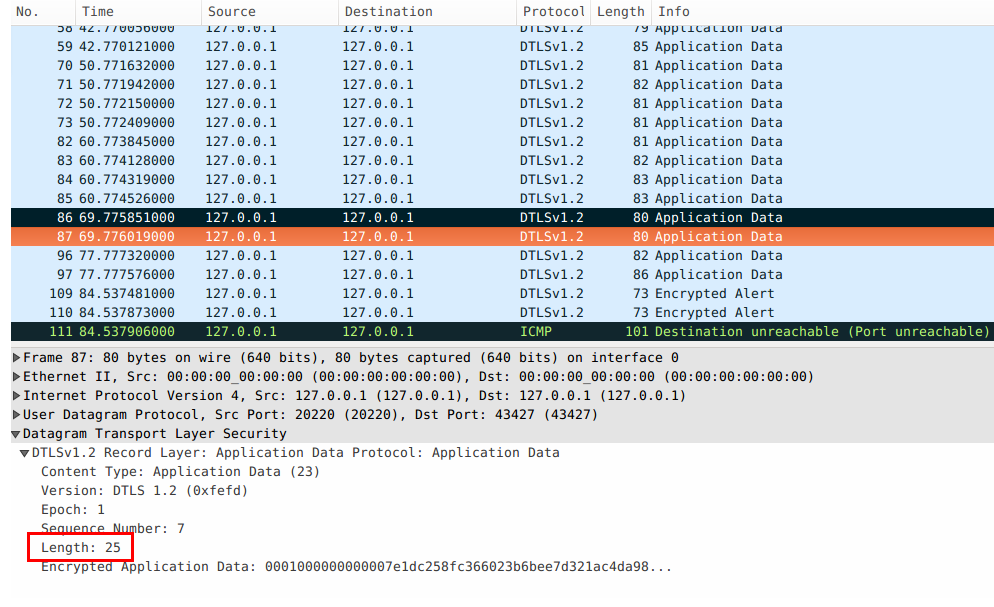
\includegraphics{./Pics/Wireshark01.png}}
\caption{Captured Leaky Coffee packets}
\label{Fig: Captured Leaky Coffee packets}
\end{figure}

\subsection{Session Detection and Segmentation}
The existence of packets implies that a session is taking place between CLIENT and SERVER.

Further more, since there is a significant difference in the timestamp intervals between continuous packets from same session and different session, one can group packets by their timestamps. Typically a threshold of $4$ seconds is good enough for \textbf{Leaky Coffee}. As we can see in the “Time” column in \Cref{Fig: Captured Leaky Coffee packets}\footnote{The in-continuous packet number is a result for filtering DTLS packets on the hosting machine.},
\begin{itemize}
\item Packet $70$ to $73$ is a session with $FlavourRequest$ and $FlavourResponse$.
\item Packet $82$ to $85$ is another session with $FlavourRequest$ and $FlavourResponse$.
\item Packet $86$ and $87$ is a session without $FlavourRequest$ and $FlavourResponse$.
\item Packet $96$ and $97$ is another session without $FlavourRequest$ and $FlavourResponse$.
\item ...
\end{itemize}

Once a session has been segmented, we can immediately label them as described in \Cref{Def: Leaky Coffee Session}.

\subsection{Plaintext Guessing} \label{Sec: Plaintext Guessing}
Similar to \textbf{Odd or Even}(\Cref{Sec: Odd or Even}), plaintexts exchanged in \textbf{Leaky Coffee} has distinguish length which could possibly be exploited to recover the plaintexts.

%
%We denote the value of DTLS Length field as $l_D$ and the actual application data length as $l$. Our experiment shows that:
%
%under both IPv4 and IPv6.
%
%\begin{definition}
%For a specific packet in a session, let $\mathbb{X}$ be the set of plaintext and $\mathbb{Y}$ be the set of its corresponding content length.
%
% We model the plaintext  and their corresponding content length (in bytes) as a channel: 
% \begin{center}
% $W(y|x), x \in \mathbb{X}, y \in \mathbb{Y}$.
% \end{center}
%
%And then the inverse of this channel $W^{-1}(x|y)$ can be viewed as the leakage channel of $\mathbb{Y}$.
%\end{definition}
%
%The general idea is that with such leakage channel, an adversary can then “decode” the plaintext using this leakage channel.
%
%In this context, $\mathbb{X}$ is the set of packet content and $\mathbb{Y}$ the set of content length $l$.
%
%\begin{example} \label{Exmp: Single-Order}
%We begin with a simple example: $Order$.
%
%For $Order$ packets, we have:
%
%\begin{table}[H]
%\begin{center}
%{\begin{tabular}{c|l|l|l||l|}
$W(y|x)$          & 5 & 8 & 9 & $P$\\
\hline
"AMERICANO" &   &  & 1  & $1/4$ \\
\hline
"CAPPUCINO" &   &   & 1  & $1/4$\\
\hline
"MOCHA"     & 1 &   &    & $1/4$\\
\hline
"ESPRESSO"  &   &  1  &   & $1/4$\\
\hline
\end{tabular}
}
%\end{center}
%\caption{Content-Length Channel and the probabilities of $Order$}
%\label{Tbl: Order1}
%\end{table}
%
%In this implementation, CLIENT randomly picks \textit{Order} from $COFFEE$; therefore the probability for every value is $1/4$. Since neither DLTS nor the application induces any randomness to the content length therefore it will always be a deterministic value.
%
%Given $W$ and the probability of $Order$, it can then compute the joint distribution of $(Order, l)$ by:
%\begin{equation}
%(\widehat{W}P)(x,y) = P(x)W(y|x)
%\end{equation}
%
%\begin{table}[H]
%\begin{center}
%{\begin{tabular}{c|c}

$\widehat{W}P$  & P     \\ \hline
("AMERICANO",9) & $1/4$ \\ \hline
("CAPPUCINO",9) & $1/4$ \\ \hline
("MOCHA",5)     & $1/4$ \\ \hline
("ESPRESSO",8)  & $1/4$ \\ \hline
\end{tabular}
}
%\end{center}
%\caption{Joint distribution of $(Order, l)$}
%\label{Tbl: Order2}
%\end{table}
%
%Then follows the marginal distribution of content length:
%\begin{equation}
%P(Y=y) = \sum\limits_{x \in \mathbb{X}}{\widehat{W}P(x,y)}
%\end{equation}
%
%\begin{table}[H]
%\begin{center}
%{\begin{tabular}{|c|c|}
\hline
 $y$ & P     \\ \hline
5 & $1/4$ \\ \hline
8 & $1/4$ \\ \hline
9 & $1/2$ \\ \hline
\end{tabular}}
%\end{center}
%\caption{Marginal distribution of $l$}
%\label{Tbl: Order3}
%\end{table}
%
%Finally we can construct the leakage channel using Bayes’ theorem:
%\begin{equation}
%P(x|y) = {\frac {P(x)P(y|x)} {P(y)}} 
%\end{equation}
%\begin{table}[H]
%\begin{center}
%{\begin{tabular}{c|c|c|c|c|}
$W^{-1}(x|y)$  & “AMERICANO” & “CAPPUCINO” & “ESPRESSO” & “MOCHA” \\ \hline
5 &             &             &            & $1$     \\ \hline
8 &             &             & $1$        &         \\ \hline
9 & $1/2$       & $1/2$       &            &         \\ \hline
\end{tabular}
}
%\end{center}
%\caption{Leakage channel of Length - $Order$}
%\label{Tbl: Order4}
%\end{table}
%
%\end{example}
%
%The same strategy can also be applied on the second packet: $Order || Flavour$.
%
%\begin{example}
%The first step is to compute the Content-Length channel. Analysis on $Order||Flavour$ packet is more complicated as it has a larger entropy. 
%
%We omit the sequence of SUGAR and MILK to simplify the problem. We also simplify our notation by denoting $D_1$ as the degree of SUGAR and $D_2$ the degree of MILK. Then any $Flavour$ can be represented as $(D_1, D_2)$, e.g. $(2,1)$ represents any $Flavour$ that has a degree of SUGAR 2 and degree of MILK 1.
%
%The same strategy can be applied directly on this example as well. However, the space of this channel is much more complicated in this case which are $4 $
%
%It is sometimes possible to simplify the problem by breaking the Plaintext-Length channel into several sub-channels, namely $Order$ channel $W_{0}(y \in l|x \in COFFEE)$, SUGAR channel $W_{1}(y \in l| x \in D_1)$ and MILK channel $W_{2}(y \in l | x \in D_2)$ in this application. These sub-channels requires less computation and we will show how to reconstruct the Plaintext-Length channel using these sub-channels later in this section. 
%
%Obviously that $W_0$ is identical to \Cref{Tbl: Order1} as the $Order$ part in $Order||Flavour$ is simply an echo of the first $Order$ packet. 
%
%$W_2$ and $W_3$ are actually identical:
%
%\begin{table}[H]
%\begin{center}
%{\begin{tabular}{c|c|c|c|c||l|}
$W_1(x|y)$ & 0 & 1 & 2 & 3 & P     \\ \hline
0          & 1 &   &   &   & $1/4$ \\ \hline
1          &   & 1 &   &   & $1/4$ \\ \hline
2          &   &   & 1 &   & $1/4$ \\ \hline
3          &   &   &   & 1 & $1/4$ \\ \hline
\end{tabular}
}
%{\begin{tabular}{c|c|c|c|c||l|}
$W_2(x|y)$ & 0 & 1 & 2 & 3 & P     \\ \hline
0          & 1 &   &   &   & $1/4$ \\ \hline
1          &   & 1 &   &   & $1/4$ \\ \hline
2          &   &   & 1 &   & $1/4$ \\ \hline
3          &   &   &   & 1 & $1/4$ \\ \hline
\end{tabular}
}
%\end{center}
%\caption{Channels of SUGAR-Length and MILK-Length}
%\label{Tbl: SUGAR-Length and MILK-Length}
%\end{table}
%
%Then we merge $W_1$ and $W_2$ to construct the $Flavour$ - Length channel $W_1 \otimes W_2((y_1, y_2) |(x_1, x_2))$ where $(y_1, y_2) \in l \otimes l, (x_1, x_2) \in D_1 \otimes D_2$:
%
%\begin{table}[H]
%\begin{center}
%{\begin{tabular}{c|c|c|c|c|c|c|c||c|}
$W_1 \otimes W_2((y_1,y_2)|(x_1, x_2))$ & (0,0) & (0,1) & ... & $(y_1, y_2)$             & ... & (3,2) & (3,3) & P         \\ \hline
(0,0)             & 1     &       &     &                          &     &       &       & $1/16$  \\ \hline
(0,1)             &       & 1     &     &                          &     &       &       & $1/16$  \\ \hline
...               &       &       &     &                          &     &       &       &           \\ \hline
$(x_1, x_2)$      &       &       &     & $P((y_1,y_2)|(x_1,x_2))$ &     &       &       & $P(x_1, x_2)$ \\ \hline
...               &       &       &     &                          &     &       &       &           \\ \hline
(3,2)             &       &       &     &                          &     & 1     &       & $1/16$  \\ \hline
(3,3)             &       &       &     &                          &     &       & 1     & $1/16$  \\ \hline
\end{tabular}}
%\end{center}
%\caption{$Flavour$-Length channel}
%\label{Tbl: Flavour channel}
%\end{table}
%
%The right end column of probability is simply the joint probability of both inputs of $W_1$ and $W_2$. 
%
%In this application, degree of SUGAR and degree of MILK are independent variables. This implies their joint probability is simply the product of their marginal probabilities:
%\begin{equation}
%P(x_1, x_2) = P(x_1) P(x_2)
%\end{equation}
%
%Notice that since the output of such channel are actually the length of its input; therefore for a given input, its output is deterministic, i.e.
%\begin{eqnarray} 
%P((y_1,y_2)|(x_1,x_2)) =
%	\begin{cases}
%	1 &\text{if } y_1 = |x_1| \text{ and } y_2 = |x_2| \\
%	0 &\text{otherwise}
%	\end{cases}
%\label{Eq: Length Probability}
%\end{eqnarray}
%
%The merged channel $W_1 \otimes W_2$ results in a table with size of $(|X_1||X_2|)$ rows and $(|Y_1| |Y_2|)$ columns. This implies that the merge operation of two channels will potentially has an exponential time and space complexity. However, this can be improved by compressing the channel.
%
%The first thing is that the merged output are actually lengths of both inputs; hence $(y_1, y_2)$ can be replaced by their sum: $y = y_1 + y_2$. Therefore \Cref{Tbl: Flavour channel} can be compressed by combing columns with a same length, i.e. we can merge columns into one if $(y_1 + y_2) = (y\prime_1 + y\prime_2)$. The combination is simply the vector sum of two columns
%
%So we can reconstruct $W_1 \otimes W_2$ as:
%\begin{table}[H]
%\begin{center}
%{\begin{tabular}{c|c|c|c|c|c|c|c||c|}
$(W_1 \otimes W_2)\prime( y =y_1 + y_2 | (x_1, x_2))$ & 0 & 1 & 2 & 3 & 4 & 5 & 6 & P      \\ \hline
(0,0)             & 1 &   &   &   &   &   &   & $1/16$ \\ \hline
(0,1)             &   & 1 &   &   &   &   &   & $1/16$ \\ \hline
...               &   &   &   &   &   &   &   &        \\ \hline
(1,0)             &  & 1 &   &   &   &   &   &        \\ \hline
...               &   &   &   &   &   &   &   &        \\ \hline
(3,2)             &   &   &   &   &   & 1 &   & $1/16$ \\ \hline
(3,3)             &   &   &   &   &   &   & 1 & $1/16$ \\ \hline
\end{tabular}}
%\end{center}
%\caption{Compressed $Flavour$-Length channel}
%\label{Tbl: Compressed Flavour}
%\end{table}
%
%In \Cref{Tbl: Compressed Flavour}, we can see that different inputs can map to the same length, e.g. $(0,1)$ and $(1,0)$ all results to $l = 1$.
%
%Practically, we can further compress this channel with the cost of resolution of input. Generally, there are some facts that worth notice:
%\begin{itemize}
%\item As in \eqref{Eq: Length Probability},  length is deterministic given a content. Therefore it is a reasonable choice to merge contents which will result into same length.
%\item The intuition of combing two rows with the same length can be interpreted as follow: for two rows with the same output $W(y| x=x_1)$ and $W(y|x=x_2)$, the merged row represents $W(y|x=x_1 \text{ or } x = x_2 )$.
%\item For such a channel, each input are exclusive events; thus the probability of the input of merged rows is simply the sum of the probability of each row: $P(x_{merged}) = P(x_1) + P(x_2)$
%\end{itemize} 
%
%So if we compress \Cref{Tbl: Compressed Flavour} by the same $(y_1 + y_2)$ which is indeed $|Flavour|$, we will have a further compressed $W_1 \otimes W_2$:
%
%\begin{table}[H]
%\begin{center}
%{\begin{tabular}{c|c|c|c|c|c|c|c||c|}
$(W_1 \otimes W_2)''(y = y_1+y_2 | x = x_1 + x_2)$ & 0 & 1 & 2 & 3 & 4 & 5 & 6 & P      \\ \hline
0                     & 1 &   &   &   &   &   &   & $1/16$ \\ \hline
1                     &   & 1 &   &   &   &   &   & $1/8$  \\ \hline
2                     &   &   & 1 &   &   &   &   & $3/16$ \\ \hline
3                     &   &   &   & 1 &   &   &   & $1/4$  \\ \hline
4                     &   &   &   &   & 1 &   &   & $3/16$ \\ \hline
5                     &   &   &   &   &   & 1 &   & $1/8$  \\ \hline
6                     &   &   &   &   &   &   & 1 & $1/16$ \\ \hline
\end{tabular}
}
%\end{center}
%\caption{Further Compressed (with less resolution) $Flavour$-Length channel }
%\label{Tbl: Further Compressed Flavour}
%\end{table}
%
%The actual degree of SUGAR and MILK are lost in \Cref{Tbl: Further Compressed Flavour} during this compression, but it also reduced the number of rows from $16$\footnote{$(W_1 \otimes W_2)\prime$ has $4 \times 4 = 16$ rows.} to $7$.
%
%By applying the same strategy again to merge the $Order$ channel $W_0$ with $(W_1 \otimes W_2)$, we will have the $OrderFlavour$-Length channel $W = W_0 \otimes W_1 \otimes W_2$. Then finally as described in \Cref{Exmp: Single-Order}, we can construct the leakage channel $W^{-1}(x|y)$ (see \Cref{OrderFlavour leakage channel}) for the $OrderFlavour$ packets .
%\end{example}
%
%To generalise, given the distribution of the plaintext, the leakage channel is constructed as following:
%\begin{description}
%\item[1] If the space of plaintext is large, break the plaintext-length channel into several sub-channels.
%\item[2] Compute the sub-channels and compress them. Resolution may lost during the compression.
%\item[3] Merge the sub-channels to construct the plaintext-length channel.
%\item[4] Use Bayes’ Theorem to invert plaintext-length channel.
%\end{description}
%
%Another aspect to view such leakage channel is to analyse its capacity, i.e. the maximum mutual information of content and length, as described in \cite{Web2}.
%
%\subsection{Guessing Plaintext Using Joint Packet Length} \label{Sec: Guessing Plaintext Using Joint Packet Length}
% In \Cref{Sec: Guessing Plaintext by One Packet Length} we described a method of packet analysis against a single packet in a session. It is possible to improve the analysis by looking at the packets jointly. As presented in \cite{Web2}, the sequence of packets lengths can be viewed as a vector.



%For example, a 2-packets session (packet No 86 and 87) has been marked out in \Cref{Fig: Captured Packets 01}. The values of DTLS Length  are both $25$ as marked in red rectangle. Their actual plaintext length can then be computed as $8$ and $8$ bytes respectively by \Cref{Eq: Plaintext length}. 
%
%It is possible to do the single packet analysis described in \Cref{Sec: Guessing Plaintext by One Packet Length} on each of these packets. We immediately know that plaintext in the first packet is “ESPRESSO”; whilst the second one could be either “ESPRESSO” or “MOCHA” with a $Flavour$ of length $3$. However, the analysis of the second packet is in fact unnecessary at all as the application specifies that an “ESPRESSO” $Order$ can only be responded with an “ESPRESSO” with NULL $Flavour$.
%
%The application specifies that the first part of the $Order||Flavour$ simply echoes the first packet; therefore in fact we can immediately tell that the second packet is “ESPRESSO”.
%\end{example}
%
%One way to model this is to “expand” the channel. Instead of using the content at each packet from as the input, we can write them as a vector:
%\begin{equation*}
%\vec{x} = <x_1, x_2, ..., x_n>
%\end{equation*}
%
%and similarly, we can also write their length as another vector:
%\begin{equation*}
%\vec{l} = <y_1, y_2, ..., y_n>
%\end{equation*}
%
%Then we can use the same strategy in \Cref{Sec: Guessing Plaintext by One Packet Length} to construct the leakage channel $W^{-1}(X, Y)$ where $\vec{x} \in X$ and $\vec{y} \in Y$. 
%
%A problem in this method is the resulting channel is of the size of the Cartesian product of all contents in every packet. However, in this Leaky Coffee application most of the cells is actually $0$ which could be used to reduce its storage space; but such optimisation is heavily application dependant.
%
%A probably better way to model this side channel is to use Hidden Markov Model\cite{baum1966} similar to \cite{Danezis_trafficanalysis}. Techniques of Machine Learning might also be able to utilise this side channel information more efficiently. However, in this “intentionally crafted” Leaky Coffee application, the first packet seems always enough to reveal (roughly) the rest of plaintext in a session.
%
%\subsection{Estimate plaintext distribution}
%In \Cref{Sec: Guessing Plaintext by One Packet Length} and \Cref{Sec: Guessing Plaintext Using Joint Packet Length} we have demonstrated how to construct a channel given the set of plaintext and their distribution. In this section, we will try to estimate the plaintext distribution by the distribution of ciphertext.
%
%The general idea is that the distribution of length (as presented as $P$ column in \Cref{Tbl: Order3}) can actually be observed from the ciphertext; therefore we can revert the process and use it to estimate the distribution of plaintext.
%
%\begin{example}
%Assume we have a sample of encrypted $Order$ packet collected where we estimated the its length distribution as following: 
%\begin{table}[H]
%\begin{center}
%{\begin{tabular}{|c|c|}
\hline
 $y$ & P     \\ \hline
5 & $d_1$ \\ \hline
8 & $d_2$ \\ \hline
9 & $d_3$ \\ \hline
\end{tabular}
}
%\end{center}
%\caption{Estimated length distribution from encrypted $Order$ packets}
%\label{Tbl: Estimated length distribution from encrypted $Order$ packets}
%\end{table}
%
%Similar to \Cref{Exmp: Single-Order}, the first step is to construct a Content-Length channel. The difference is that this time we do not have the pre-knowledge of plaintext distribution; therefore we represent the content distribution as unknown variables $p_i$ for each content.
%
%\begin{table}[H]
%\begin{center}
%{\begin{tabular}{c|l|l|l||l|}
$W(y|x)$          & 5 & 8 & 9 & $P$\\
\hline
"AMERICANO" &   &  & 1  & $p_1$ \\
\hline
"CAPPUCINO" &   &   & 1  & $p_2$\\
\hline
"MOCHA"     & 1 &   &    & $p_3$\\
\hline
"ESPRESSO"  &   &  1  &   & $p_4$\\
\hline
\end{tabular}
}
%\end{center}
%\caption{Content-Length Channel with unknown distibution of $Order$}
%\label{Tbl: Content-Length Channel with unknown distibution of $Order$}
%\end{table}
%
%
%%Since we are only interested in $p_1$ and $p_3$ and the appearance of each content is exclusive, \Cref{Tbl: Content-Length Channel with unknown distibution of $Order$} can be rewritten as \Cref{Tbl: Rewritten Content-Length Channel with unknown distibution of $Order$}.
%%
%%\begin{table}[H]
%%\begin{center}
%%{\begin{tabular}{c|c|c|c||c|}
$W(y|x)$          & 5 & 8 & 9 & $P$\\
\hline
"AMERICANO" &   &  & 1  & $p_1$ \\
\hline
"MOCHA"     & 1 &   &    & $p_3$\\
\hline
"ESPRESSO" or "CAPPUCINO"  &   &  $p_4 / (p_2 + p_4)$  &  $p_2 / (p_2 + p_4)$  & $p_4 + p_2$\\
\hline
\end{tabular}
}
%%\end{center}
%%\caption{Rewritten Content-Length Channel with unknown distibution of $Order$}
%%\label{Tbl: Rewritten Content-Length Channel with unknown distibution of $Order$}
%%\end{table}
%
%Their joint distribution follows immediately.
%
%\begin{table}[H]
%\begin{center}
%{\begin{tabular}{c|c}

$\widehat{W}P$  & P     \\ \hline
("AMERICANO",9) & $p_1$ \\ \hline
("CAPPUCINO",9) & $p_2$ \\ \hline
("MOCHA",5)     & $p_3$ \\ \hline
("ESPRESSO",8)  & $p_4$ \\ \hline
\end{tabular}
}
%\end{center}
%\caption{Joint distribution of $(Order, l)$ with unknown distribution of $Order$}
%\label{Tbl: Joint distribution of $(Order, l)$ with unknown distribution of $Order$}
%\end{table}
%
%Then we can compute the marginal distribution of length.
%
%\begin{table}[H]
%\begin{center}
%{\begin{tabular}{|c|c|}
\hline
 $y$ & P     \\ \hline
5 & $p_3$ \\ \hline
8 & $p_4$ \\ \hline
9 & $p_1 + p_2$ \\ \hline
\end{tabular}}
%\end{center}
%\caption{Marginal distribution of $l$ with unknown distribution of $Order$}
%\label{Tbl: Marginal distribution of $l$ with unknown distribution of $Order$}
%\end{table}
%
%By linking \Cref{Tbl: Marginal distribution of $l$ with unknown distribution of $Order$} with \Cref{Tbl: Estimated length distribution from encrypted $Order$ packets} we have the following constrains to the content distribution:
%
%\begin{equation} \label{Eq: Plaintext Distribution Estimation}
%\left \{
%\begin{aligned}
%p_3 = d_1\\
%p_4 = d_2\\
%p_1 + p_2 = d_3\\
%\sum\limits_{i = 1}^4{p_i} = 1
%\end{aligned}
%\right
%\end{equation}
%
%Any solution satisfies \Cref{Eq: Plaintext Distribution Estimation} can be viewed as a reasonable guess to the distribution of the contents.
%
%\end{example}

\chapter{Plan}

The short term plan is to finish the toy application analysis in \Cref{Chp: Progress To Date}. There are these directions in this task:
\begin{enumerate}
\item So far we have mainly focused on demonstrating the phenomenon similar to those described in \cite{Web1} and \cite{Web2} exists in our set up, but there could possibly be more. For example, it is probably worth study whether it is feasible to deduce the plaintext distribution in \Cref{Sec: Leaky Coffee} given encrypted packets.
\item To see if the attacks in \Cref{Sec: Leaky Coffee} can be optimised.
\item Apply and evaluate some countermeasures to these attacks.
\item Only a few, nearly none, attempt has been made to study types of attack other than \cite{Web1} and \cite{Web2}; hence this might also be worth trying.
\end{enumerate}

One of the greatest deficiency in the work so far is the risk of being alienated from reality since the toy applications are designed in an extremely abstracted way whilst the real world application could be much more complicated and will not be intentionally designed to be vulnerable to attacks. Therefore as a long term plan, it is very important to get in touch with some actual application and evaluate those we have developed from the toys. Having said so, one of the greatest challenges is  the immaturity of IoT; hence following the trend of related technologies would be an important and constant task in this project.
\chapter{Other Activities}

I have been one of the TAs for Cryptography A and System Security during the first term of 2014 - 2015. 

I also attended Real World Crypto 2015.

\appendix
\chapter{OrderFlavour-Length leakage channel}
\label{OrderFlavour leakage channel}

In this application, the joint probability of $Order$ and $Flavour$ are simply the product of their marginal probability. However, since “ESPRESSO” will always followed by $Flavour$ of of both degree of SUGAR and MILK being $0$(see  \Cref{ESPRESSO}); hence
\begin{eqnarray*}
P(x_1, x_2 | \text{“ESPRESSO”}) = 
	\begin{cases}
	1 &\text{if } x_1 = x_2 = 0\\
	0 &\text{otherwise}
	\end{cases}
\end{eqnarray*}

Therefore
\begin{eqnarray*}
P(\text{“ESPRESSO”}, x_1, x_2 ) = 
	\begin{cases}
	1/4 &\text{if } x_1 = x_2 = 0\\
	0 &\text{otherwise}
	\end{cases}
\end{eqnarray*}


%\bibliographystyle{ieeetran}
%\bibliography{references,rfc}
\printbibliography

\end{document}